\documentclass[../main.tex]{memoir}

\begin{document}

\chapter{Características espacio-temporales para la detección de
  acciones anómalas}
\label{sec:model-analysis}

En este capítulo estudiaremos el uso de características
espacio-temporales para la detección de acciones anómalas en vídeo.
Concretamente, tomaremos como punto de partida el modelo propuesto en
el trabajo \textit{Real-World Anomaly Detection in Surveillance
  Videos} \cite{sultani2018real}, y realizaremos una propuesta de
mejora. Nuestro enfoque consiste en cambiar el extractor de
características empleado originalmente, el cual se basa en el uso de
convoluciones 3D \cite{tran2015learning}, por uno basado en
convoluciones clásicas 2D seguido de una etapa recurrente.\\

Nuestra hipótesis defiende que, aunque las convoluciones 3D están
pensadas para extraer información de fragmentos de vídeo, no son
capaces de capturar correctamente la dependencia temporal a largo
plazo. La falta de capacidad en este sentido produce un empeoramiento
global del modelo, el cual puede subsanarse con un extractor de
características más potente, que haga uso tanto de capas
convolucionales para extraer información espacial como de capas
recurrentes para aprender la secuencia temporal.\\

En esta sección se detallará la experimentación llevada a cabo,
describiendo el conjunto de datos utilizado, el modelo original,
y las modificaciones propuestas.

\section{Conjunto de datos empleado: UCF-Crime Dataset}

El conjunto de datos con el que se ha trabajado fue propuesto por los
propios autores del artículo que estamos estudiando\footnote{Puede
  consultarse la página del proyecto en
  \url{https://www.crcv.ucf.edu/projects/real-world/}}. Dicho conjunto
de datos está compuesto por secuencias de vídeo extraídas de cámaras
de videovigilancia. Según puede consultarse en la página del proyecto,
la base de datos está compuesta por 1900 vídeos de longitud variable,
con una media de 7247 fotogramas. Estamos hablando, por tanto, de
vídeos de una longitud aceptable, de varios minutos de media. En
total, se dispone de 128 horas de vídeo, y se incluyen 13 clases
distintas de anomalías, así como vídeos que se consideran normales. Se
consideran vídeos normales aquellos en los que no aparecen
comportamientos anómalos. Algunas de las clases de anomalía que se
incluyen en el conjunto son abusos, robos, allanamientos de morada,
tiroteos, asaltos a comercios, peleas o explosiones.\\

Una particularidad del conjunto de datos es la gran diversidad de
entornos en los que se recogen los vídeos. En la figura
\ref{fig:ucf-normal-examples} se pueden observar distintos fotogramas
extraídos de vídeos normales. Como se puede apreciar, tenemos vídeos
tomados por cámaras interiores y exteriores, tanto a la luz del día
como por la noche, y con distintos ángulos de cámara. Esto limita la
posibilidad de hacer asunciones sobre los datos, y obliga a construir
un modelo genérico, capaz de funcionar en diversas situaciones.

\begin{figure}[hbtp]
  \centering
  \begin{subfigure}{0.48\textwidth}
    \centering
    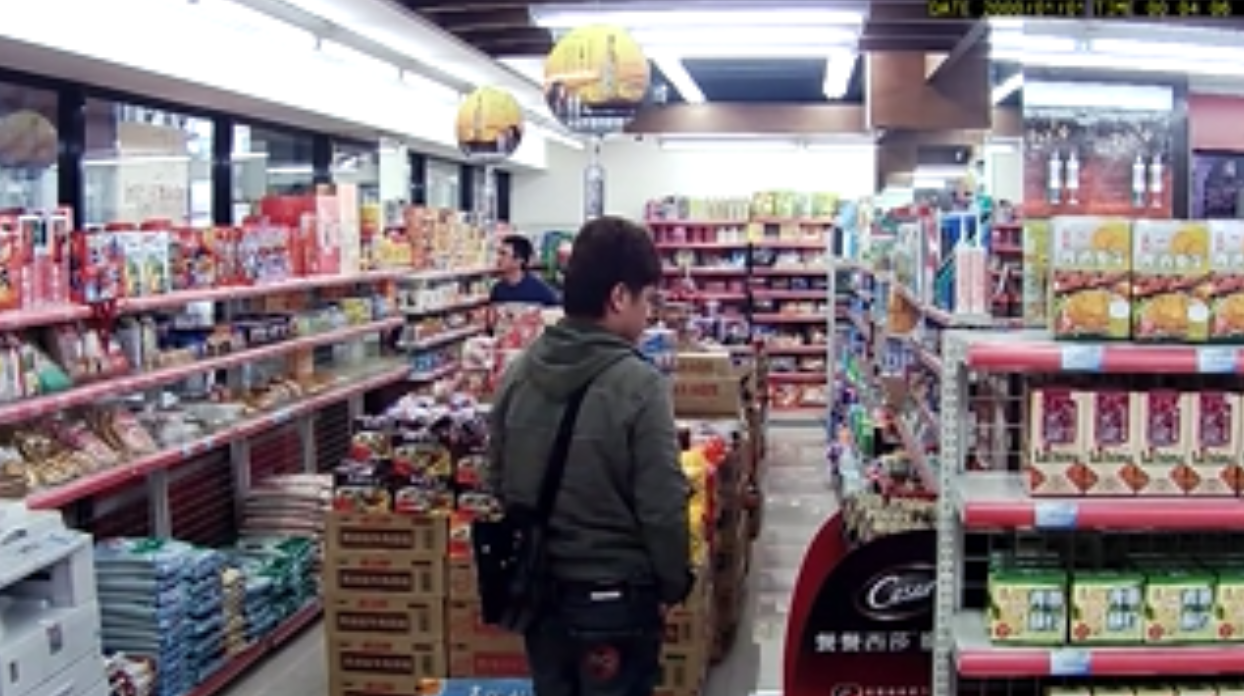
\includegraphics[width=\linewidth]{images/ucf-examples/normal-1}
    \caption{Interior a la altura de la vista}
  \end{subfigure}
  \begin{subfigure}{0.48\textwidth}
    \centering
    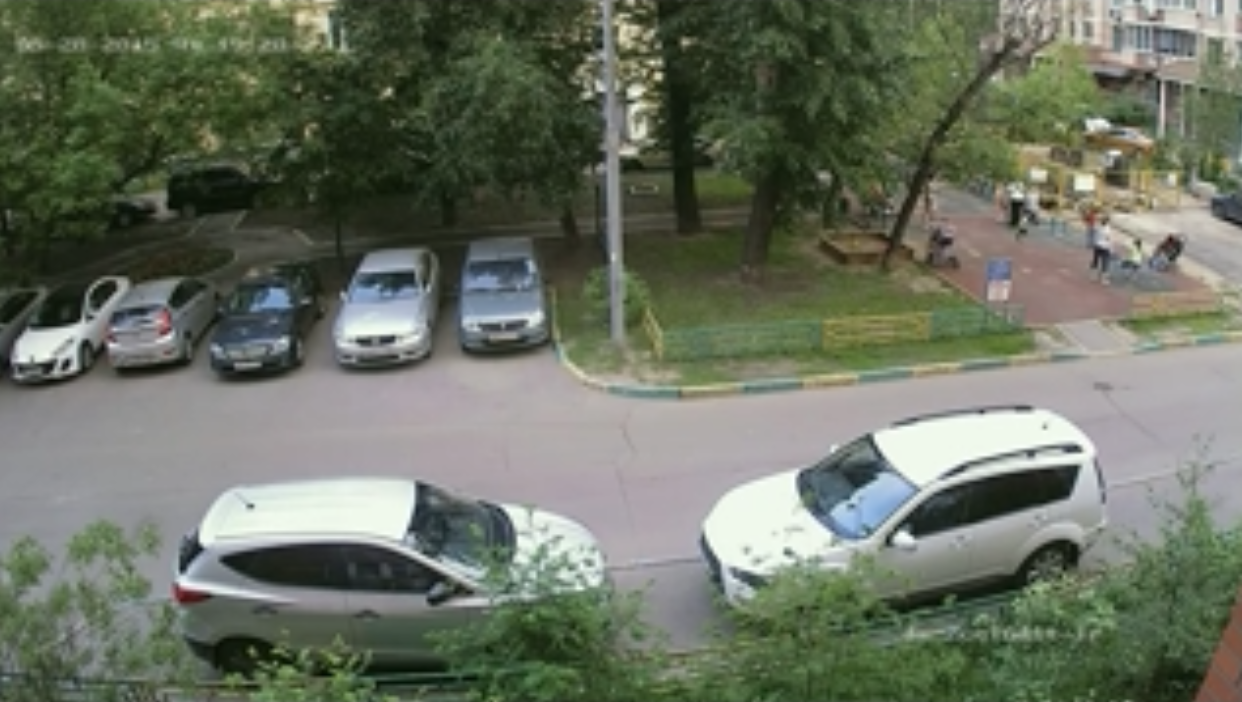
\includegraphics[width=\linewidth]{images/ucf-examples/normal-2}
    \caption{Exterior de día}
  \end{subfigure}
  \begin{subfigure}{0.48\textwidth}
    \centering
    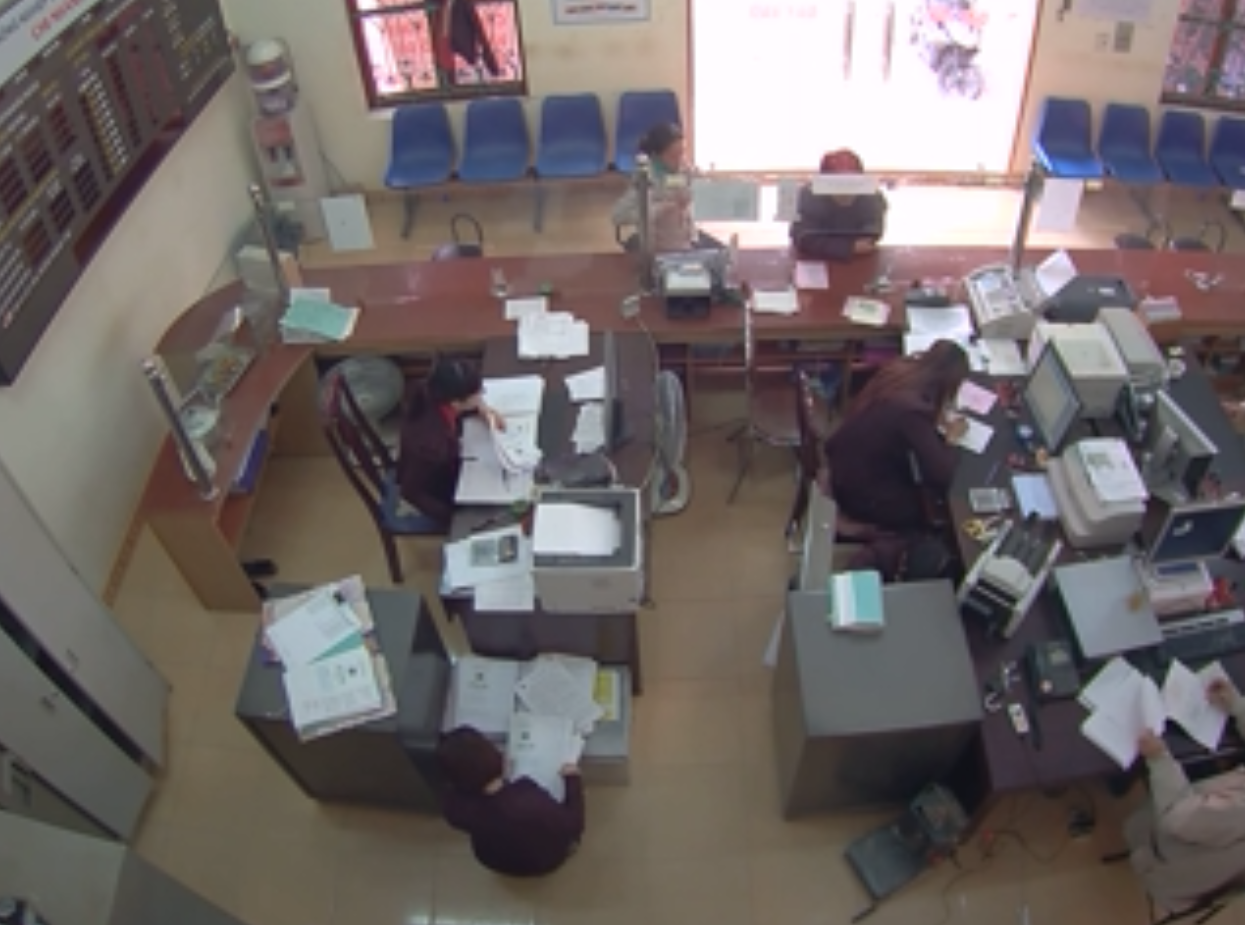
\includegraphics[width=\linewidth]{images/ucf-examples/normal-3}
    \caption{Interior desde arriba}
  \end{subfigure}
  \begin{subfigure}{0.48\textwidth}
    \centering
    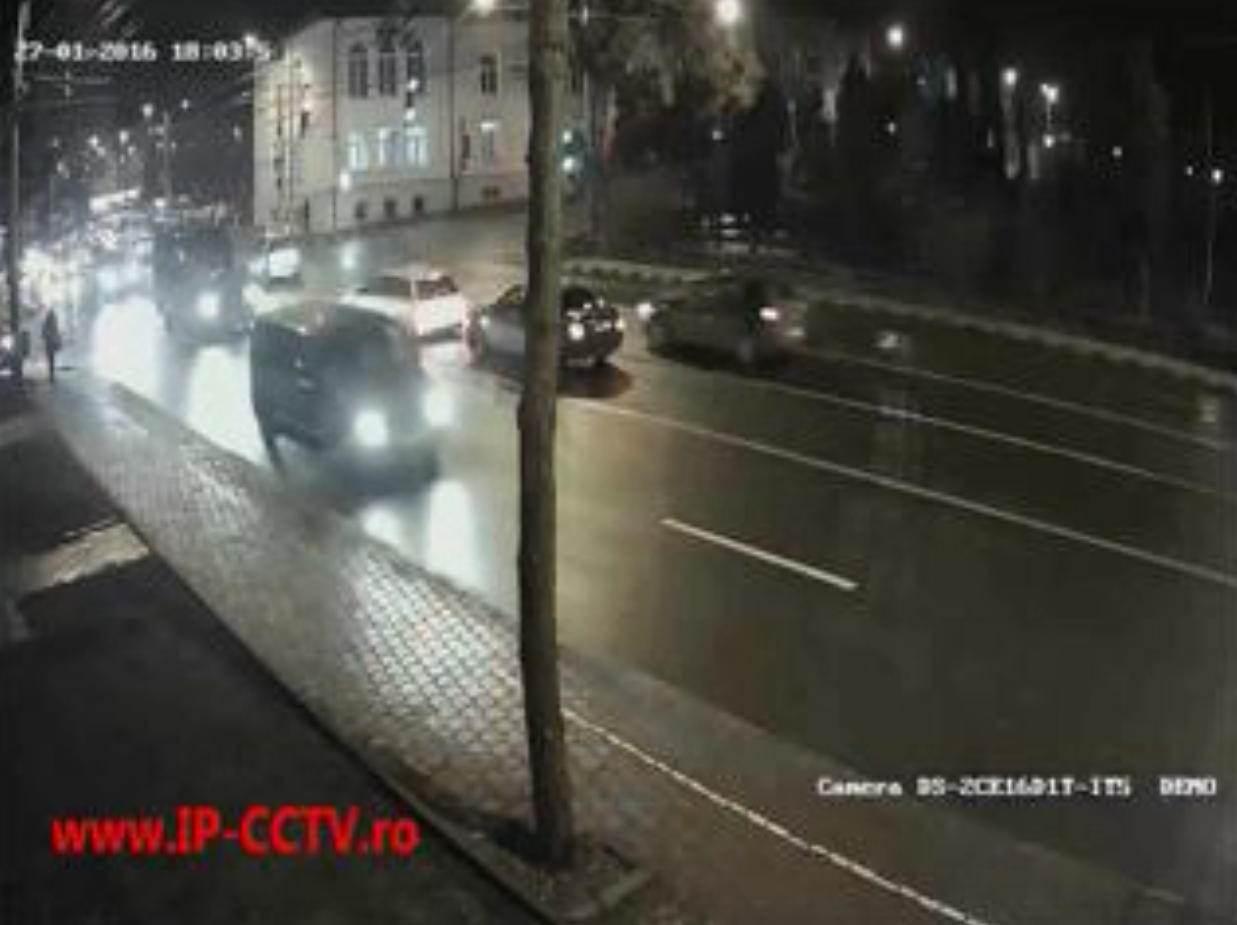
\includegraphics[width=\linewidth]{images/ucf-examples/normal-4}
    \caption{Exterior de noche}
  \end{subfigure}
  \caption{Ejemplos de fotogramas normales del conjunto de datos
    UCF-Crime. Podemos observar la gran variabilidad de las escenas
    del conjunto.}
  \label{fig:ucf-normal-examples}
\end{figure}

Se proponen dos problemas distintos. Por un lado, se pide diseñar un
modelo que sea capaz de marcar cuándo ocurre una anomalía (es decir,
un problema binario, en el que se debe marcar para cada fotograma del
conjunto de datos si presenta o no anomalía), y por otro, para los
vídeos etiquetados como anómalos, asignar correctamente la clase a la
que pertenecen. En nuestro caso, nos centraremos en resolver el
primero de los problemas. Los autores del modelo original dan mucha
más importancia a la primera parte que a la segunda, y por tanto
nosotros nos hemos centrado en su análisis, ignorando la segunda
parte. Por tanto, para nosotros no habrá distinción entre las
distintas clases de anomalías, por lo que a partir de este momento
sólo haremos la distinción entre vídeos normales y anómalos. El
conjunto de datos está dividido en subconjuntos de entrenamiento y
test. Para el conjunto de entrenamiento se dispone de 800 vídeos
normales y 810 vídeos anómalos. Para el conjunto de datos de test, se
dispone de 290 vídeos (150 normales, 140 anómalos).\\

La principal particularidad del conjunto de datos es que el
subconjunto de entrenamiento está débilmente etiquetado. Esto
significa que, aunque el objetivo a abordar consista en localizar
temporalmente cuándo ocurre una anomalía, las etiquetas de las que se
dispone en el conjunto de entrenamiento sólo marcan que el vídeo es
anómalo, no dónde ocurre dicha anomalía. Por tanto, en lugar de tener
para cada vídeo un valor binario por fotograma indicando si hay una
anomalía o no presente en dicho fotograma, lo que se tiene es una
única etiqueta binaria para el vídeo completo. Como se puede observar
en la figura \ref{fig:ucf-anomaly-examples}, en los vídeos que presentan
anomalía hay también una parte importante del vídeo correspondiente a
fotogramas normales.\\

\begin{figure}[hbtp]
  \centering
  \begin{subfigure}{0.48\textwidth}
    \centering
    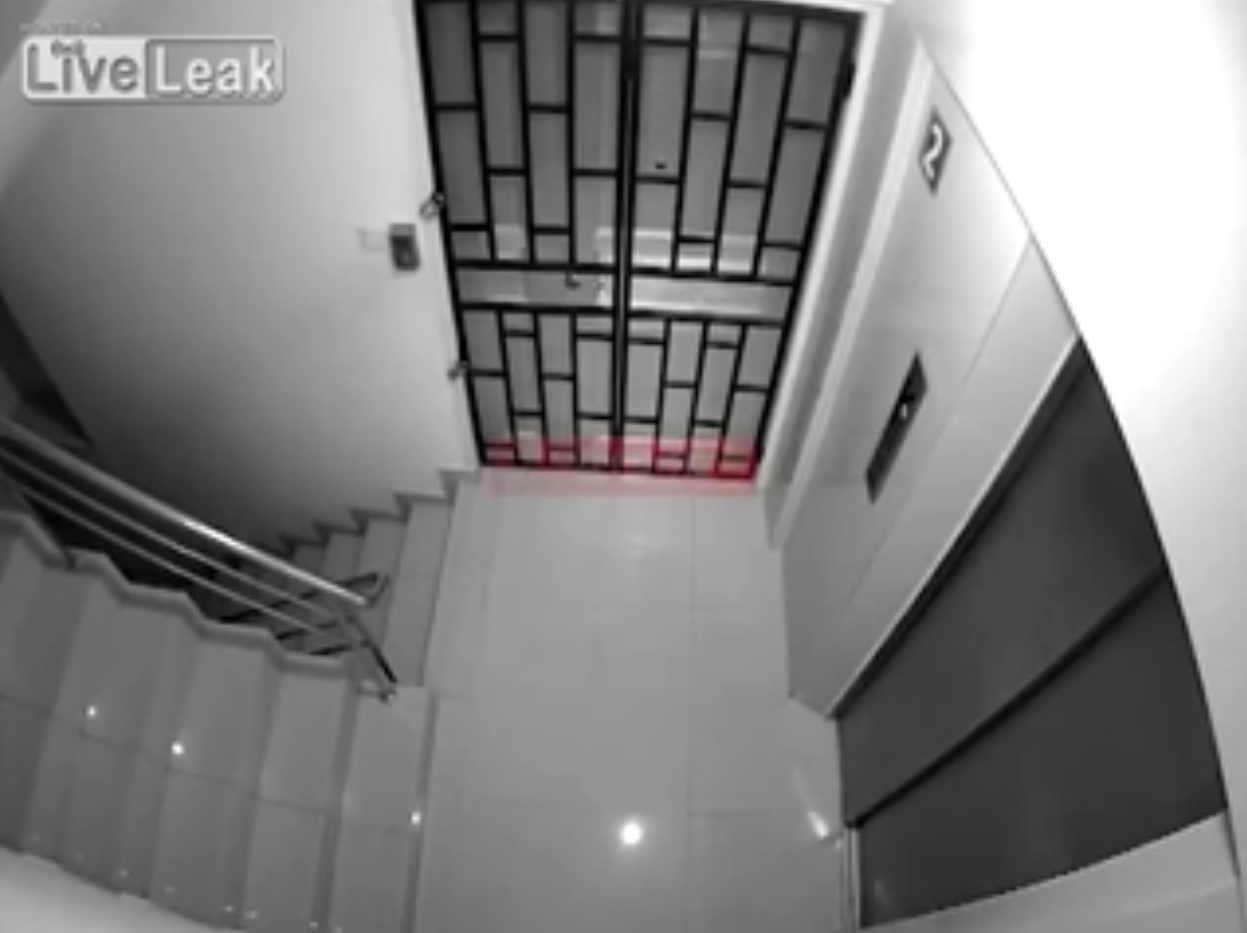
\includegraphics[width=\linewidth]{images/ucf-examples/arson-normal}
    \caption{Fuego - Fotograma normal}
  \end{subfigure}
  \begin{subfigure}{0.48\textwidth}
    \centering
    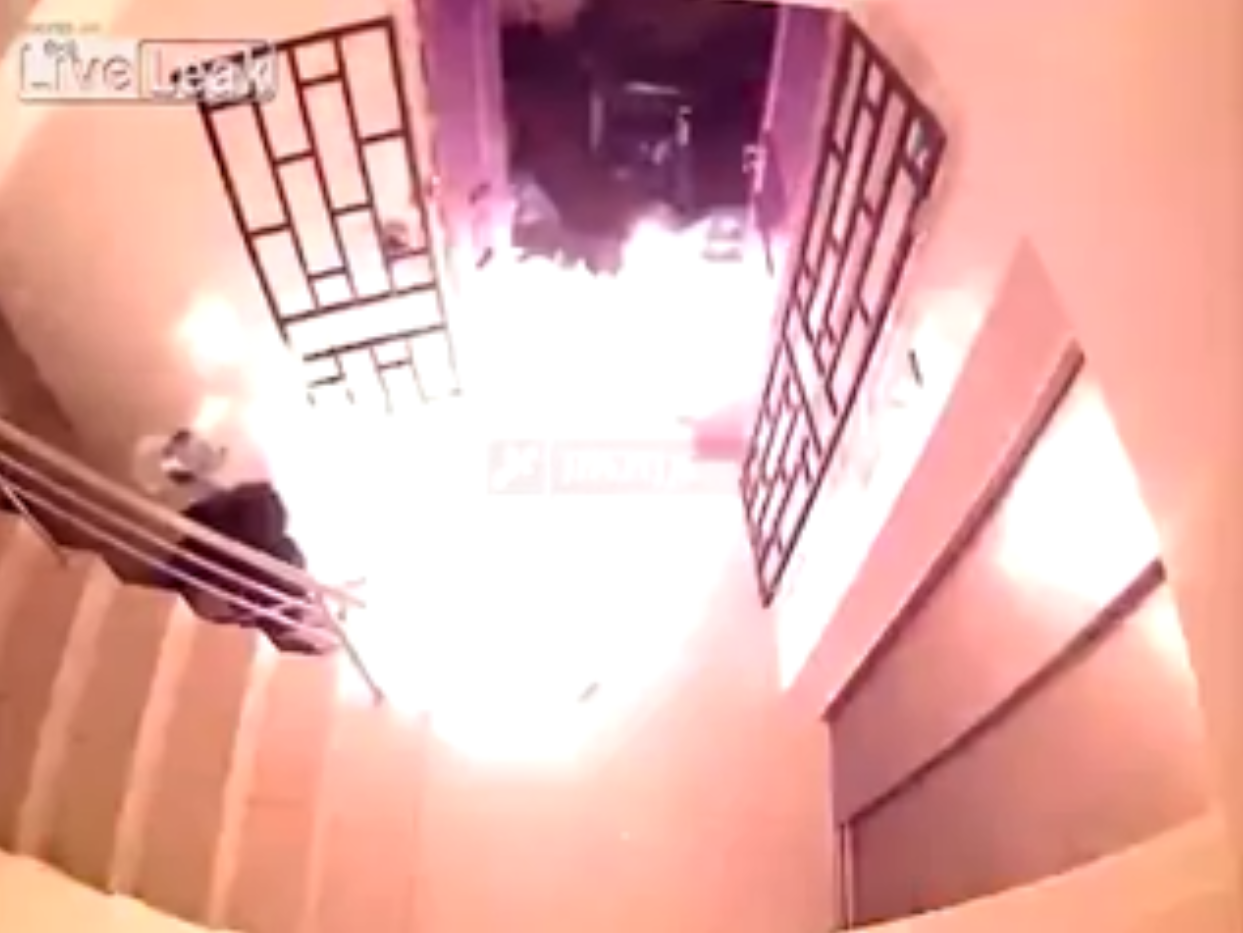
\includegraphics[width=\linewidth]{images/ucf-examples/arson-abnormal}
    \caption{Fuego - Fotograma anómalo}
  \end{subfigure}
  \begin{subfigure}{0.48\textwidth}
    \centering
    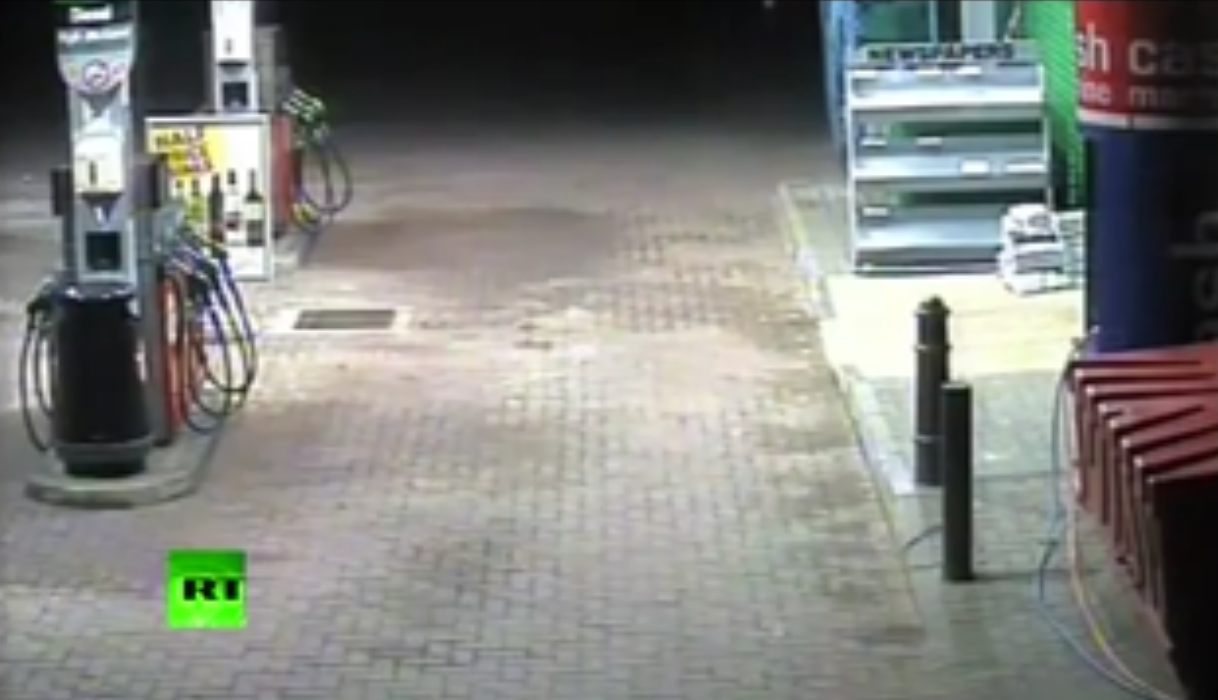
\includegraphics[width=\linewidth]{images/ucf-examples/explosion-normal}
    \caption{Explosión - Fotograma normal}
  \end{subfigure}
  \begin{subfigure}{0.48\textwidth}
    \centering
    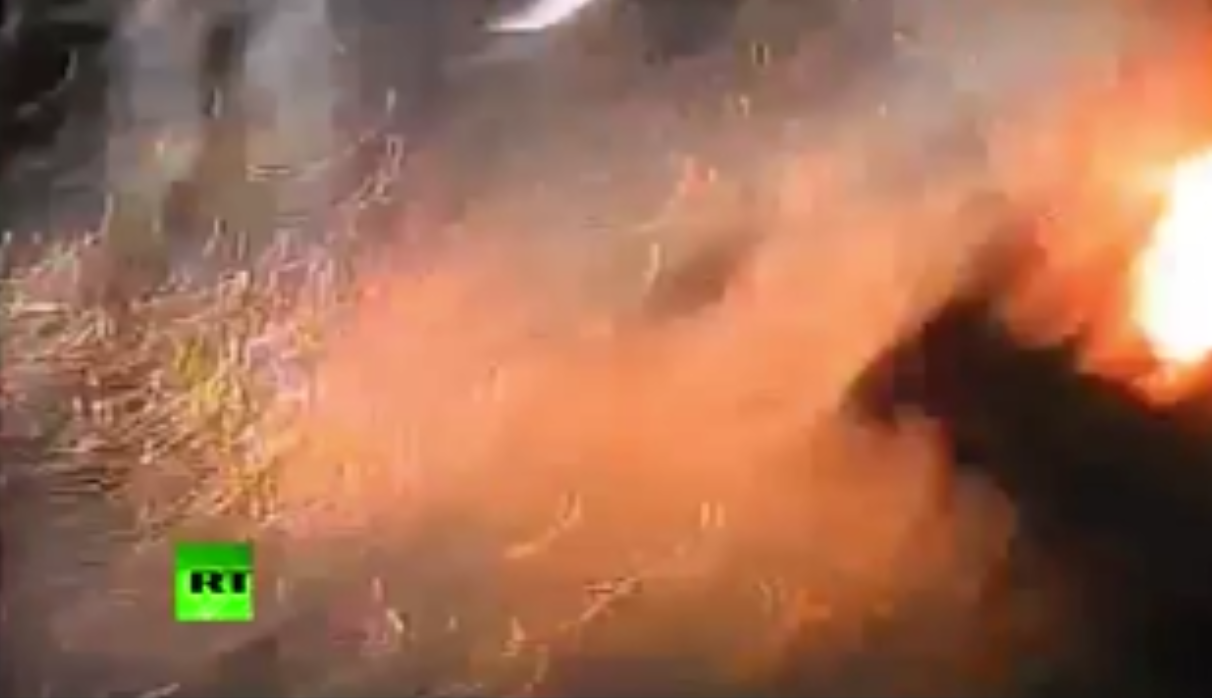
\includegraphics[width=\linewidth]{images/ucf-examples/explosion-abnormal}
    \caption{Explosión - Fotograma anómalo}
  \end{subfigure}
  \begin{subfigure}{0.48\textwidth}
    \centering
    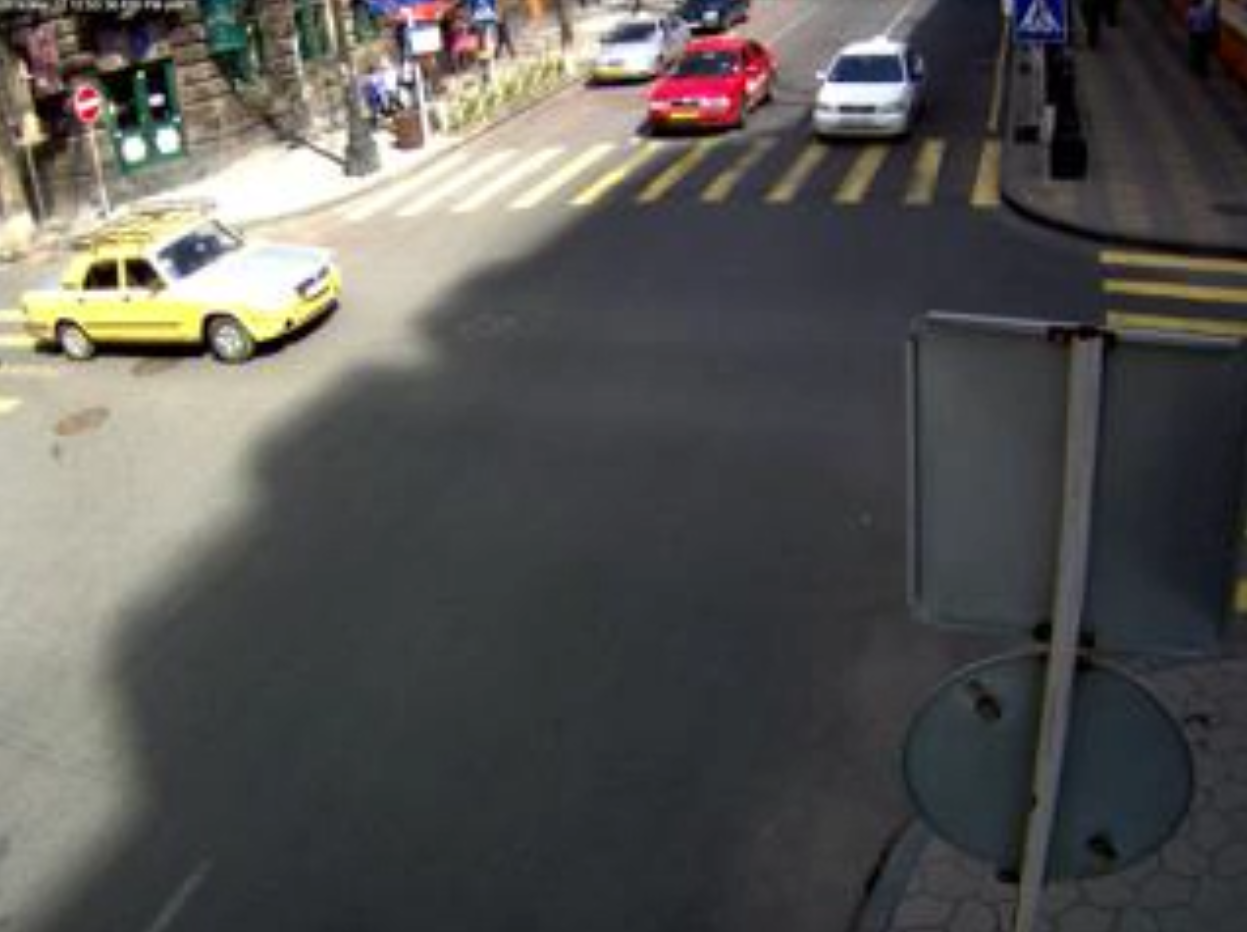
\includegraphics[width=\linewidth]{images/ucf-examples/roadaccident-normal}
    \caption{Accidente de tráfico - Fotograma normal}
  \end{subfigure}
  \begin{subfigure}{0.48\textwidth}
    \centering
    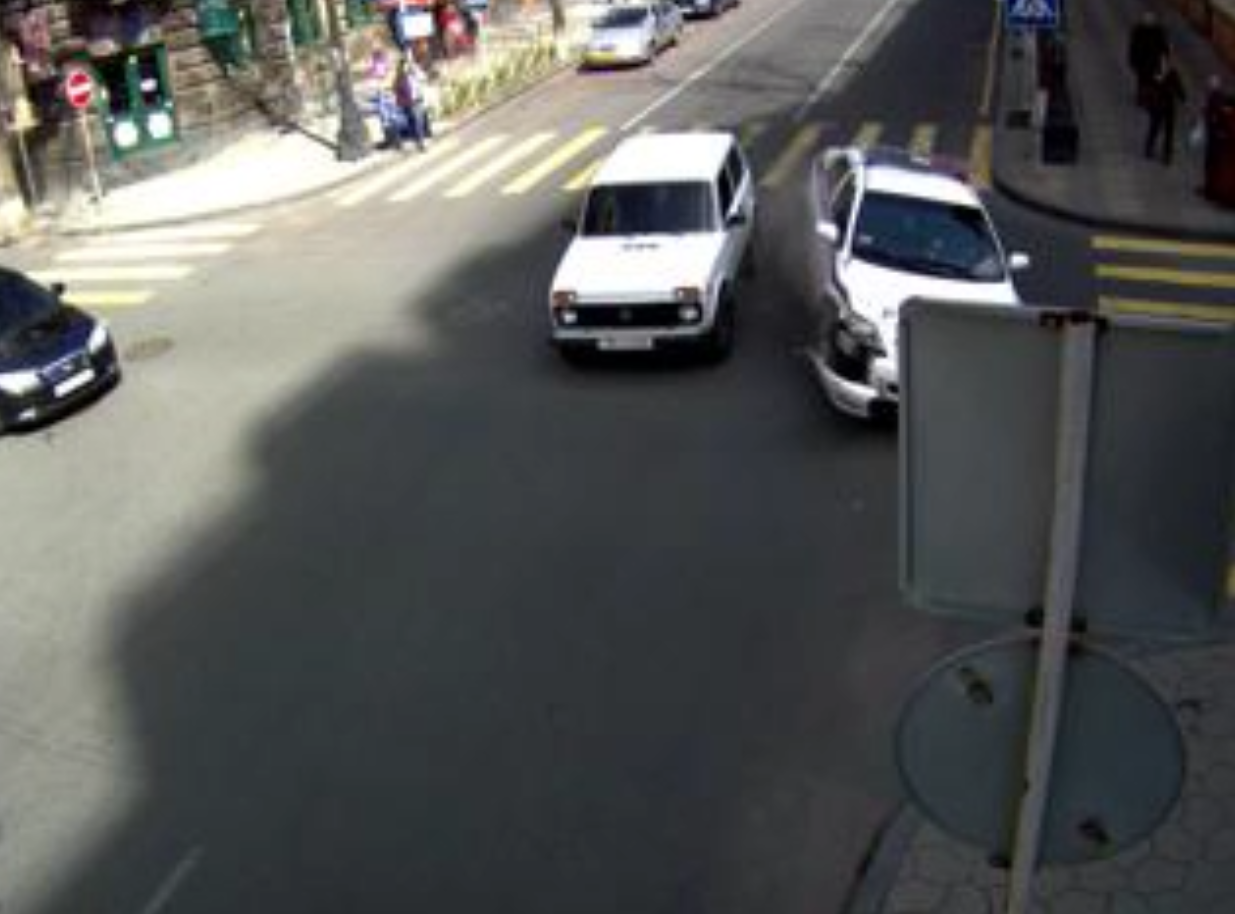
\includegraphics[width=\linewidth]{images/ucf-examples/roadaccident-abnormal}
    \caption{Accidente de tráfico - Fotograma anómalo}
  \end{subfigure}
  \begin{subfigure}{0.48\textwidth}
    \centering
    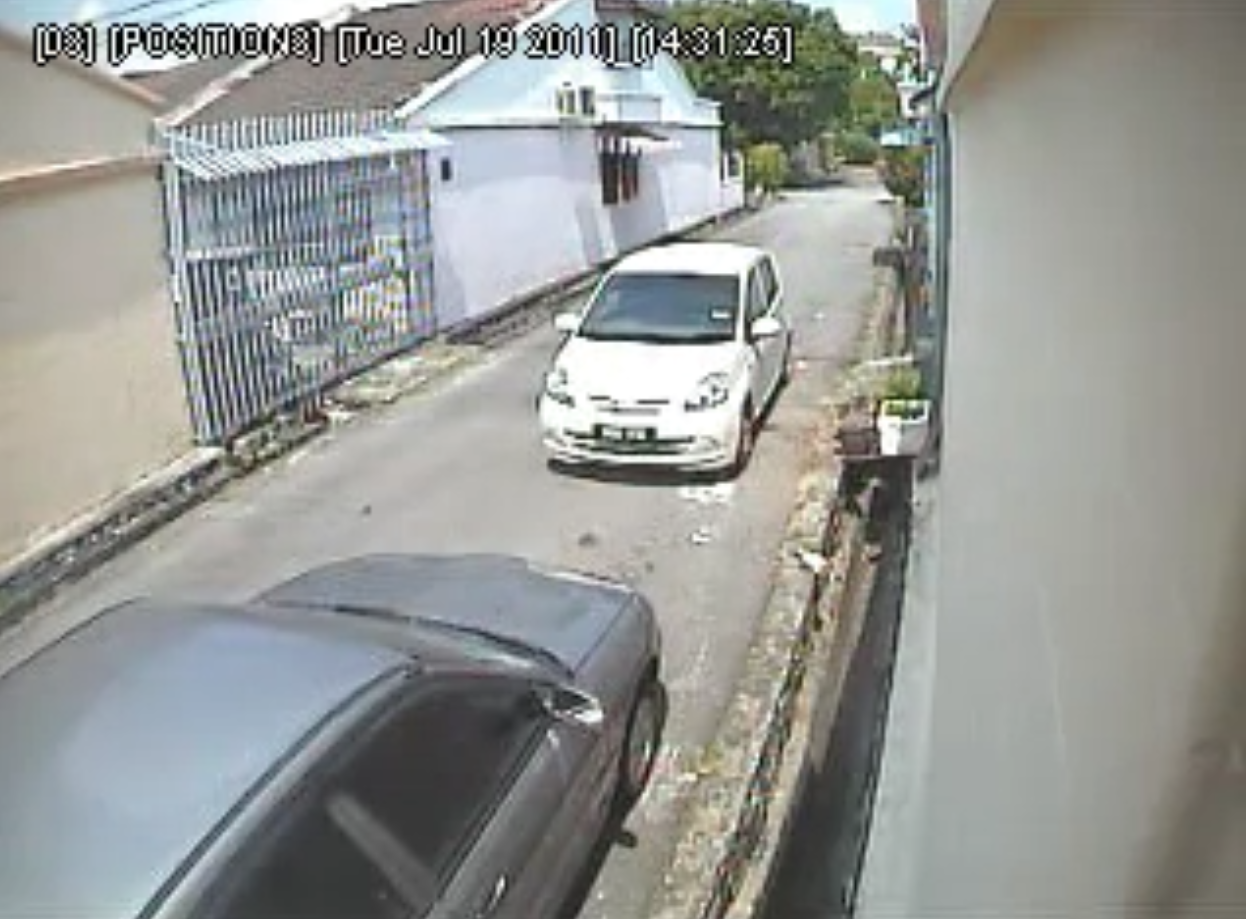
\includegraphics[width=\linewidth]{images/ucf-examples/stealing-normal}
    \caption{Robo - Fotograma normal}
  \end{subfigure}
  \begin{subfigure}{0.48\textwidth}
    \centering
    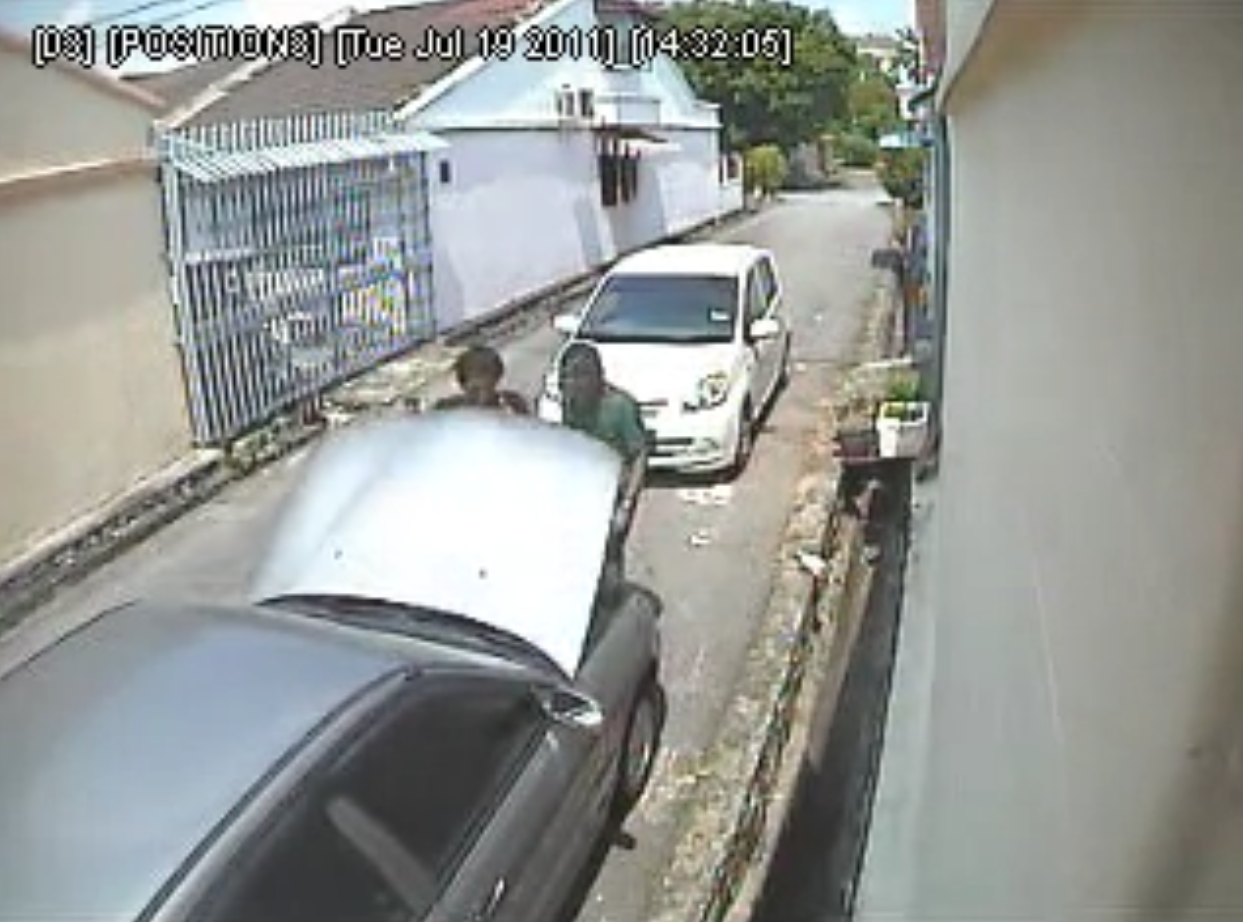
\includegraphics[width=\linewidth]{images/ucf-examples/stealing-abnormal}
    \caption{Robo - Fotograma anómalo}
  \end{subfigure}
  \caption{Ejemplos de anomalías del conjunto de datos UCF-Crime. Como
    puede observarse en cada pareja de fotogramas, en los vídeos
    anómalos hay también fragmentos normales presentes.}
  \label{fig:ucf-anomaly-examples}
\end{figure}

En el conjunto de test, sin embargo, el etiquetado es a nivel de
fotograma, y por tanto tendremos que aprender a localizar
temporalmente la anomalía en un fragmento de mayor longitud. Esto hace
que haya que diseñar un sistema de aprendizaje específico, que permita
aprender a nivel de fotograma cuando no tenemos dicha información
disponible.\\

Sobre las etiquetas del conjunto de test, observamos que nos
encontramos ante un problema fuertemente desbalanceado. En total,
disponemos de 1027477 fotogramas etiquetados como fotogramas normales,
mientras que sólo hay 84331 fotogramas anómalos. Resulta sorprendente
el hecho de que, a pesar de tener los conjuntos prácticamente
balanceados en términos de vídeos anómalos y normales, cuando
realizamos el cálculo a nivel de fotograma, existe un desbalanceo muy
importante. Esto se debe a que, en realidad, los vídeos que presentan
una anomalía concentran la misma en unos pocos segundos, y la mayoría
del tiempo de vídeo está compuesto por fotogramas normales.\\

A continuación describiremos el modelo original, así como la política
de entrenamiento del mismo.

\section{Modelo original}

En esta sección se va a describir la arquitectura original empleada.
Dicha arquitectura consiste en un extractor de características basado
en redes neuronales convolucionales en tres dimensiones, seguido por
una red completamente conectada que realiza la clasificación
final. Además, la principal aportación del modelo es una función de
pérdida que permite aprender el etiquetado a nivel de fotograma a
pesar de entrenar con etiquetado a nivel de vídeo. Esta función
resuelve la particularidad del etiquetado del conjunto de datos de
entrenamiento de forma débil.\\

En las siguientes secciones describiremos en detalle cada una de las
partes de la red, así como la función de pérdida propuesta.

\subsection{Extractor de características: C3D}

El extractor de características empleado en el modelo original es el
modelo conocido como C3D \cite{tran2015learning}. La particularidad de
este modelo es que en lugar de utilizar convoluciones en dos
dimensiones, que son las que suelen usarse típicamente en el
tratamiento de imágenes, se utilizan convoluciones en tres
dimensiones. La diferencia radica en que la convolución en dos
dimensiones sólamente desplaza el kernel a lo largo del ancho y el
alto de la imagen. El núcleo de convolución es, por tanto, una matriz,
y la salida de la convolución es en dos dimensiones.\\

Cuando se aplica una convolución 3D, se tiene en cuenta también la
dimensión temporal. En este caso, los núcleos son tensores de rango 3,
y la convolución no utiliza un único fotograma, si no que tiene en
cuenta varios fotogramas consecutivos. De esta forma, no sólo se
recoge información espacial (en las dimensiones alto y ancho), sino
que también se recoge información temporal (dado que se involucra la
dimensión tiempo). Así, la salida es en tres dimensiones, en lugar de
en dos. En la imagen \ref{fig:2d-3d-conv} puede observarse
gráficamente la diferencia entre una convolución en dos dimensiones y
una convolución en tres dimensiones.\\

El extractor propuesto consiste, por tanto, en una serie de
convoluciones 3D que toman como entrada un vídeo y extraen
características del mismo.

\begin{figure}[H]
  \centering
  \begin{subfigure}{0.48\textwidth}
    \centering
    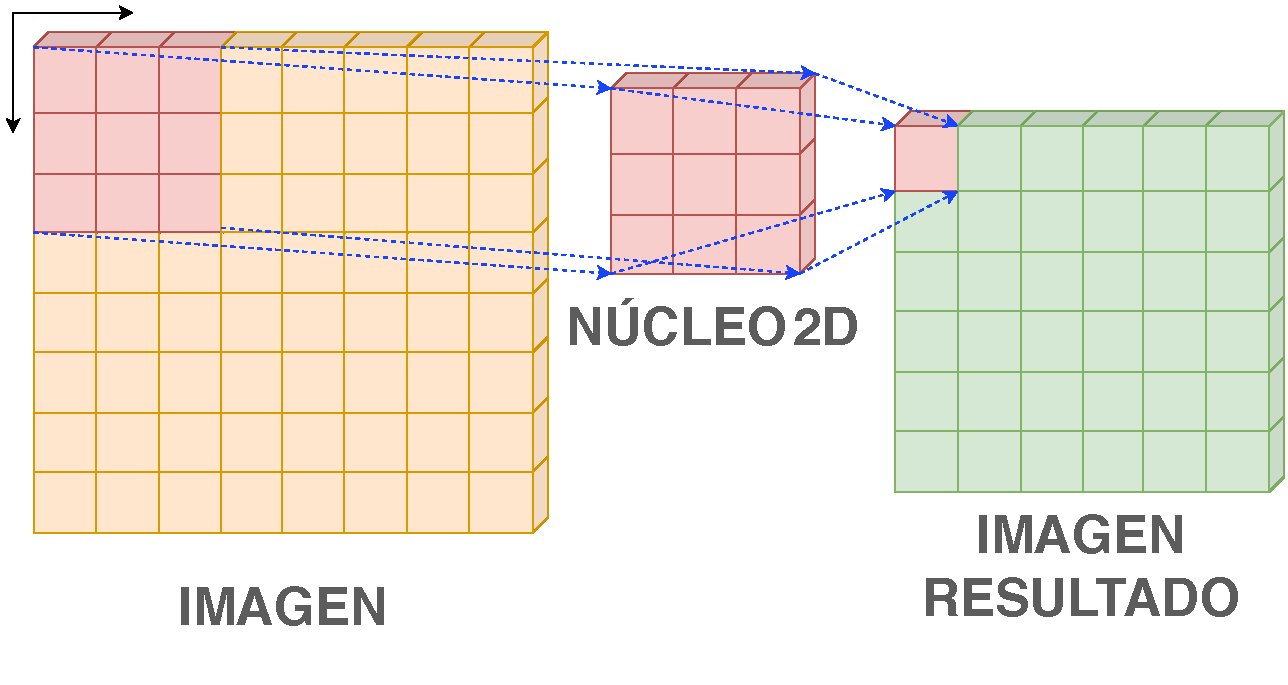
\includegraphics[width=.9\linewidth]{images/2d_conv.pdf}
    \caption{Convolución 2D}
  \end{subfigure}
  \begin{subfigure}{0.48\textwidth}
    \centering
    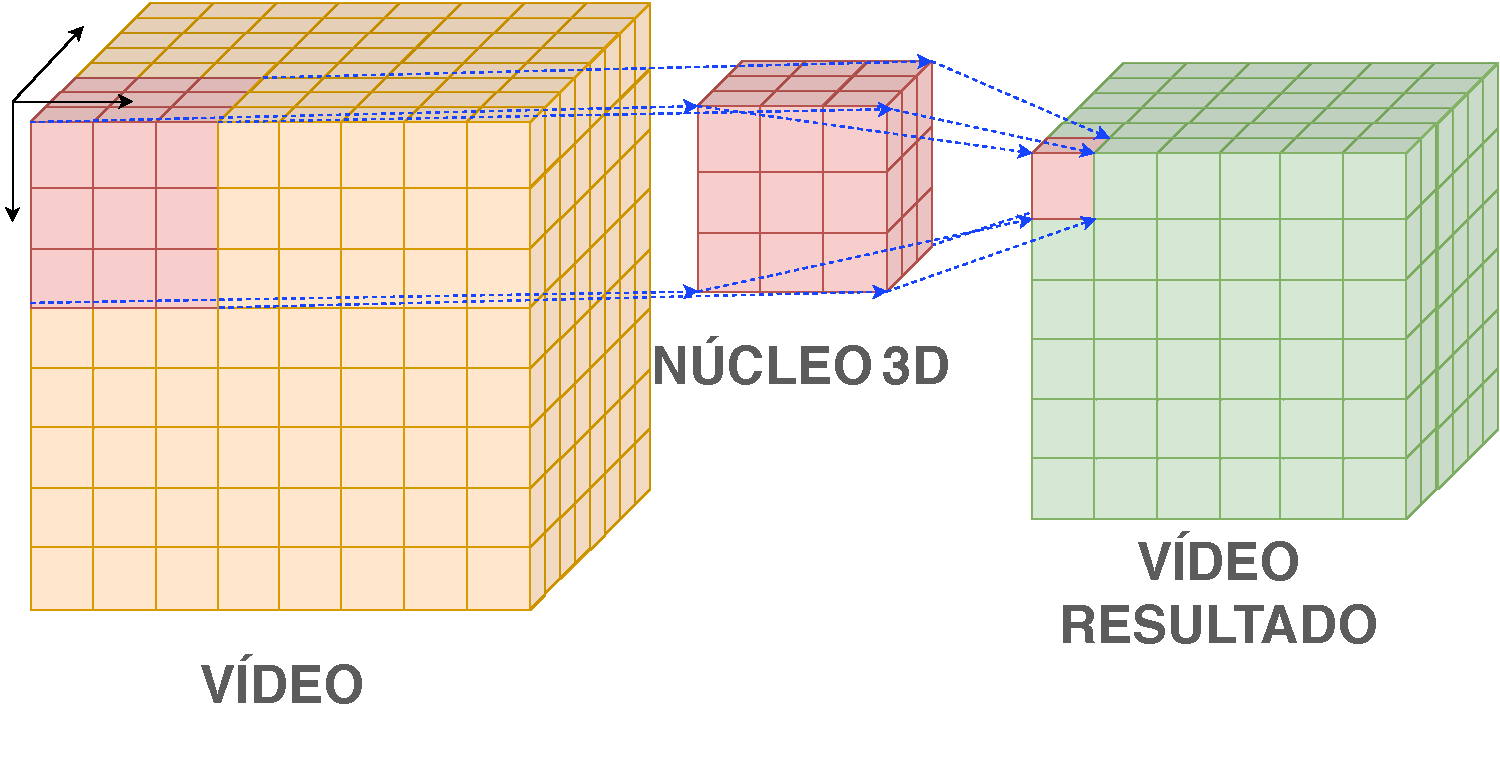
\includegraphics[width=.9\linewidth]{images/3d_conv.pdf}
    \caption{Convolución 3D}
  \end{subfigure}
  \caption{Diferencia entre la convolución en dos y en tres
    dimensiones. Como puede observarse en la imagen, en la convolución
    2D el filtro es una matriz que se desplaza en dos dimensiones. En
    la convolución 3D, por el contrario, el filtro es 3D y se mueve
    también en la dimensión temporal.}
  \label{fig:2d-3d-conv}
\end{figure}

En concreto, la arquitectura del modelo C3D es la siguiente:

\begin{itemize}
\item Convolución 3D, núcleo $3 \times 3 \times 3$, 64 filtros
\item Pooling 3D, reducción de factor 2 en las dimensiones espaciales,
  sin reducción en la dimensión temporal
\item Convolución 3D, núcleo $3 \times 3 \times 3$, 128 filtros
\item Pooling 3D, reducción de factor 2 en las tres dimensiones
\item Convolución 3D, núcleo $3 \times 3 \times 3$, 256 filtros
\item Convolución 3D, núcleo $3 \times 3 \times 3$, 256 filtros
\item Pooling 3D, reducción de factor 2 en las tres dimensiones
\item Convolución 3D, núcleo $3 \times 3 \times 3$, 512 filtros
\item Convolución 3D, núcleo $3 \times 3 \times 3$, 512 filtros
\item Pooling 3D, reducción de factor 2 en las tres dimensiones
\item Convolución 3D, núcleo $3 \times 3 \times 3$, 512 filtros
\item Convolución 3D, núcleo $3 \times 3 \times 3$, 512 filtros
\item Pooling 3D, reducción de factor 2 en las tres dimensiones
\item Capa completamente conectada, 4096 neuronas
\item Capa completamente conectada, 4096 neuronas
\item Capa de activación \textit{softmax}
\end{itemize}

Según los autores del modelo, la salida de la primera capa
completamente conectada es la que debe utilizarse como representación
del fragmento de vídeo. La entrada del modelo es un vídeo de 16
fotogramas de tamaño $112 \times 112$, y devuelve como resultado
un descriptor de 4096 elementos de dicho fragmento de vídeo.

\subsubsection{Preentrenamiento del modelo: Sports-1M Dataset}

El extractor de características empleado en el trabajo se entrena
previamente en un conjunto de datos cuyo objetivo es la clasificación
de comportamientos. Este conjunto de datos de gran tamaño suele
utilizarse como punto de partida para el entrenamiento de modelos
dedicados la extracción de características en vídeo, de forma similar
al uso de ImageNet para imágenes.\\

Dado que las redes neuronales utilizadas en trabajos de esta
envergadura suelen necesitar de conjuntos de datos de gran tamaño para
ser entrenadas, los conjuntos que se utilizan normalmente no son
suficientemente grandes para que el aprendizaje sea suficientemente
rico. Por este motivo, suele emplearse una etapa de entrenamiento
previa sobre un conjunto de datos de gran tamaño, con el que se
aprenden características genéricas, y después se afina el modelo en el
conjunto de datos con el que se trabaja. Esta técnica es la que se
conoce como transferencia de aprendizaje (\textit{Transfer learning}).\\

En concreto, en el trabajo que estamos analizando se entrena el
extractor de características en el conjunto de datos Sports-1M
\cite{karpathy2014large}. Dicho conjunto está formado por 1133158
vídeos, con un total de 487 clases distintas. El extractor de
características se entrena colocando una capa densamente conectada al
final de la arquitectura anterior, con tantas neuronas como clases
tiene el conjunto de datos (487 en este caso), y entrenando la red
completa para resolver la tarea de clasificación. Una vez entrenada la
red para resolver dicho problema, debido a que los comportamientos
presentes en el conjunto de datos son muy variados, las capas de la
red son capaces de extraer información muy diversa de los vídeos de
entrada. Para construir el extractor de características final, se
elimina la última capa de clasificación y se mantienen los pesos
aprendidos para el resto de capas. Esta última técnica es lo que
se conoce como congelar la red.\\

Tras este entrenamiento, obtenemos un modelo capaz de resumir la
información de un vídeo de 16 fotogramas en un vector de 4096
componentes. Se utilizará este modelo para resumir la información de
cada vídeo del conjunto en fragmentos de 16 fotogramas. De esta forma,
por cada vídeo, tendremos un número variable de descriptores
extraídos. En la siguiente sección analizaremos cómo se convierten
dichos descriptores en una representación de tamaño fijo del vídeo, y
como puede utilizarse esa información para entrenar el clasificador
final. Para ello, tendremos que definir una función de coste que nos
permita aprender a nivel de fotograma (o de unos pocos de fotogramas),
a pesar de tener etiquetas sólo a nivel de vídeo.

\subsection{Aprendizaje multi-instancia}

En esta sección se presenta la política de aprendizaje diseñada en el
artículo para el entrenamiento del modelo. Como hemos comentado
anteriormente, tenemos etiquetas a nivel de vídeo, pero no a nivel de
fotograma, que es la tarea que realmente queremos resolver.\\

La propuesta de entrenamiento se basa en lo que se conoce como
aprendizaje multi-instancia. En lugar de recibirse una etiqueta para
cada elemento del conjunto de datos, se recibe una bolsa con elementos
etiquetados de forma única. En el caso de la clasificación binaria,
una bolsa estará etiquetada como negativa si todos los elementos que
la conforman son elementos negativos. Por otro lado, una bolsa tendrá
etiqueta positiva si al menos uno de sus elementos es positivo. Esto
se traslada de forma muy sencilla a nuestro escenario. En nuestro
caso, cada vídeo representará una única bolsa, etiquetada como
negativa si procede de un vídeo normal (en el que no ocurren
anomalías), y positiva procede de un vídeo anormal (sabemos que ocurre
una anomalía en dicho vídeo, pero no dónde). Para conseguir una
representación de tamaño fijo para cada vídeo, se dividen los mismos
en 32 segmentos temporales, lo que hace que en cada bolsa haya 32
elementos. Para definir lo que ocupa cada segmento, se reparten de
forma equiespaciada los fragmentos de 16 fotogramas procesados
anteriormente, de forma que en cada segmento haya el mismo número de
fragmentos, todos ellos consecutivos (o el reparto más equitativo
posible, si la división no es exacta). La representación del segmento
es la media de las representaciones de los fragmentos que lo
forman. De esta forma, para cada vídeo se obtienen
32 elementos distintos, que conformarán la bolsa en cuestión.\\

Ahora, tenemos que definir la función de pérdida con la que entrenar
el modelo, dadas las bolsas que hemos obtenido. En un contexto normal,
si tuviéramos ejemplos de vídeos anómalos $\mathcal{V}_a$ y normales
$\mathcal{V}_n$ etiquetados completos, querríamos conseguir un modelo
cuya salida fuese una puntuación de anomalía, tal que

\[ f(\mathcal{V}_a) > f(\mathcal{V}_n). \]

No obstante, lo que tenemos son bolsas de ejemplos, en lugar de vídeos
completos. En dichas bolsas sabemos que existen ejemplos positivos,
pero no sabemos cuáles son. Dadas dos bolsas de ejemplos, una
proveniente de un vídeo normal $\mathcal{B}_n$ y una proveniente de un
vídeo anómalo $\mathcal{B}_a$, querremos conseguir que la puntuación
del segmento de puntuación más alta de la bolsa normal (aquel trozo de
vídeo que siendo normal resulta difícilmente clasificable) sea más
alto que el segmento de puntuación más alta de la bolsa anormal (aquel
segmento de la bolsa anómala con una probabilidad mayor de ser
anómalo). Es decir, nuestra intención será forzar que

\[ \max_{i \in \mathcal{B}_a}{f(\mathcal{V}^i_a)} > \max_{i \in
    \mathcal{B}_n}{f(\mathcal{V}^i_n)}. \]

Con esta formulación, queremos conseguir que los fragmentos que
contienen realmente una anomalía tengan una puntuación mayor que
aquellos que no la contienen, pero que son ejemplos difícilmente
clasificables. Utilizando una idea similar a la función de pérdida de
Hinge (Hinge loss), la cual se utiliza en el entrenamiento de las SVM
para maximizar el margen de clasificación, se define la función de
pérdida para el entrenamiento del modelo como

\[ l(\mathcal{B}_a, \mathcal{B}_n) = \max{(0, 1 - \max_{i \in
      \mathcal{B}_a}{f(\mathcal{V}^i_a)} + \max_{i \in
      \mathcal{B}_n}{f(\mathcal{V}^i_n)})}. \]

Además, en la función anterior hemos ignorado la estructura temporal
del vídeo de entrada. En un vídeo con anomalías, tenemos que la
mayoría del tiempo nos encontramos con fotogramas normales. Por este
motivo, queremos que la mayoría de las predicciones que hagamos sean
cercanas a cero. Además, nos interesa evitar que el cambio en la
puntuación de anomalías sea excesivamente abrupto, por lo que buscamos
que el aumento de dicho valor entre un segmento y el siguiente no sea
demasiado fuerte. Esto nos lleva a añadir dos términos de
regularización a la función de coste, que se encarguen de controlar
las dos cantidades que hemos mencionado. Con dicha modificación, la
función de pérdida final se convierte en

\begin{align*}
  l(\mathcal{B}_a, \mathcal{B}_n) &= \max{(0, 1 - \max_{i \in
                                    \mathcal{B}_a}{f(\mathcal{V}^i_a)} + \max_{i \in
                                    \mathcal{B}_n}{f(\mathcal{V}^i_n)})}\\
                                  & + \lambda_1
                                    \sum_{i=0}^{n-1} (f(\mathcal{V}_a^i) - f(\mathcal{V}_a^{i+1})) +
                                    \lambda_2 \sum_{i=0}^{n} f(\mathcal{V}_a^i).
\end{align*}

El término que acompaña al parámetro $\lambda_1$ hace referencia al
término de regularización temporal, y el término que acompaña al
parámetro $\lambda_2$ hace referencia a la regularización dispersa.
Los valores $\lambda_1$ y $\lambda_2$ pueden ajustarse para dar más
o menos importancia a los términos de regularización.\\

Una vez hemos visto la política de entrenamiento del modelo
clasificador, pasamos a dar la descripción completa del modelo
original.

\subsection{Modelo original completo}

Una vez hemos visto el extractor de características y la política de
entrenamiento, pasamos a ver cómo se entrena el modelo original
completo.\\

En la figura \ref{fig:original-model} se puede observar la estructura
completa del modelo original. Dados dos vídeos del conjunto de datos,
uno normal y uno anómalo, se extraen sus 32 segmentos temporales y se
conforman las bolsas de ejemplos. Los 32 segmentos se procesan con el
extractor de características preentrenado, y se extraen los
descriptores resumen para cada segmento. Dichos descriptores se
clasifican utilizando una red completamente conectada, la cual tiene
como única salida una neurona. Dicha neurona aprende a devolver una
puntuación de anomalía para cada segmento. Cuando se han calculado las
puntuaciones de anomalía para los vídeos positivo y negativo, se
calcula el valor de la función de pérdida y se actualizan los pesos de
las capas densas utilizando un método de descenso del gradiente. El
extractor de características está preentrenado y congelado, por lo que
en tiempo de entrenamiento del modelo completo no se actualizan sus
pesos.\\

\begin{figure}[hbtp]
  \centering
  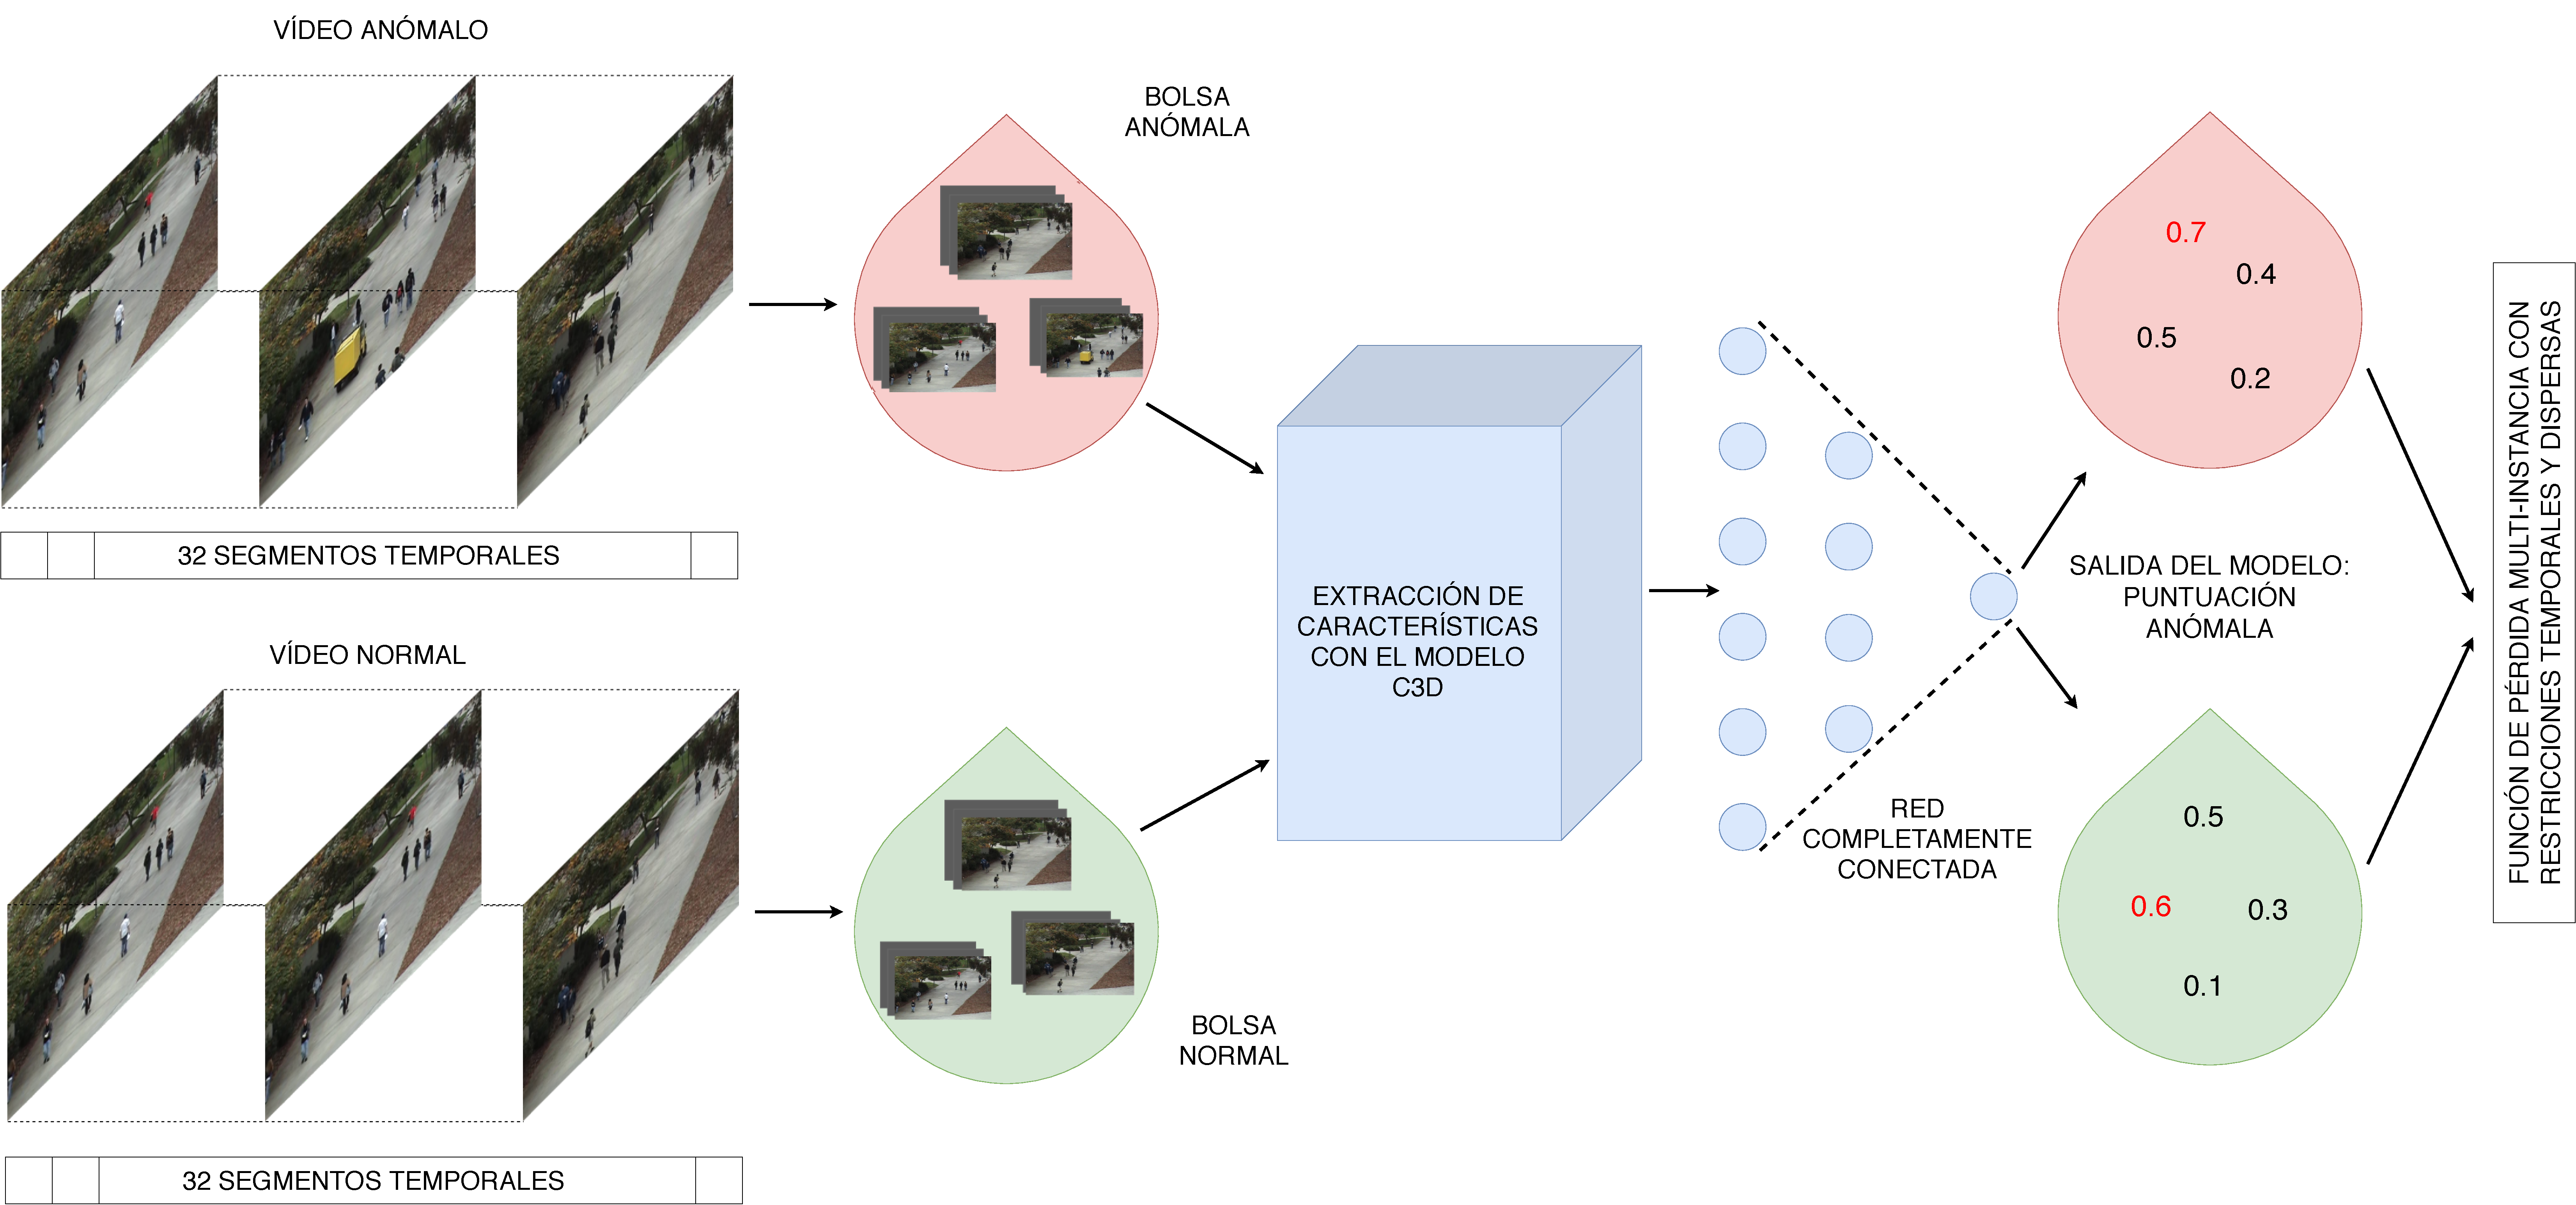
\includegraphics[width=\textwidth]{images/original_model.pdf}
  \caption{Arquitectura completa del modelo original}
  \label{fig:original-model}
\end{figure}

Para cada etapa de entrenamiento, se seleccionan aleatoriamente 60
vídeos del conjunto de forma balanceada (30 normales y 30 anómalos), y
se calcula el gradiente de la función de pérdida en función de la
clasificación de los 60 vídeos.\\

Una vez que se tiene el modelo entrenado con el sistema anterior, en
tiempo de inferencia se divide el vídeo a clasificar de la misma forma
que en entrenamiento, y se calcula la puntuación de anomalía para cada
segmento. Para obtener una predicción para cada fotograma, se
interpola la predicción de los segmentos.\\

Una vez hemos visto el modelo original al completo, pasamos a describir
la modificación propuesta.

\section{Propuesta de mejora del modelo}

La propuesta de mejora del modelo consiste en una modificación del
extractor de características por un sistema que capture correctamente
la información temporal contenida en los fragmentos de vídeo.\\

La principal crítica que se puede hacer al modelo anterior radica en
que el extractor de características no es el idóneo. A pesar de que
las convoluciones en tres dimensiones son modelos pensados para la
extracción de características en vídeo, su capacidad de extraer
información temporal contenida en un número elevado de fotogramas
consecutivos es limitada, ya que el campo receptivo de la red viene
limitado por el tamaño de los núcleos utilizados. En el caso del
modelo anterior, trabajamos con núcleos de tamaño 3, por lo que
extraeremos información que esté expresada en tres fotogramas
consecutivos, no a mayor distancia. Gracias la operación de
\textit{Pooling}, en capas más avanzadas de la red se extrae
información de fotogramas que sí se encuentran a mayor distancia, pero
en nuestra opinión la dependencia temporal está infrarrepresentada en
estos modelos.\\

Nuestra propuesta, por tanto, trata de solucionar esta problemática
proponiendo un extractor de características espacio-temporales de
mayor calidad, el cual se expone a continuación:

\subsection{Extractor de características: Xception-LSTM}

Como hemos comentado anteriormente, propuesta se basa en modificar el
extractor de características del modelo anterior, de tal forma que se
utilice una arquitectura con capacidad de capturar correctamente la
información temporal. Para ello, haremos uso de redes neuronales
recurrentes. Este tipo de modelos se distinguen de las redes
neuronales clásicas en el hecho de que conectan la salida de neuronas
de una capa con entradas de neuronas dentro de la misma capa. De esta
forma, la predicción que realizan no depende sólo de un único elemento
(o un conjunto pequeño de elementos) del vector de entrada, sino
también de la información que ha recibido la red en etapas
anteriores. En la figura \ref{fig:networks} se puede observar la
distinción entre una red neuronal clásica y una red recurrente. En
particular, utilizaremos redes convolucionales en dos dimensiones para
extraer información de todos los fotogramas del vídeo, y crearemos una
serie temporal con dichos descriptores. La serie temporal será
utilizada como entrada para una red recurrente que aprenderá el patrón
temporal.\\

\begin{figure}[hbtp]
  \centering
  \begin{subfigure}{\textwidth}
    \centering
    \begin{tikzpicture}[shorten >=1pt,->,draw=black!50, node distance=\layersep]
      \tikzstyle{every pin edge}=[<-,shorten <=1pt]
      \tikzstyle{neuron}=[circle,fill=black!25,minimum size=17pt,inner sep=0pt]
      \tikzstyle{input neuron}=[neuron, fill=green!50];
      \tikzstyle{output neuron}=[neuron, fill=red!50];
      \tikzstyle{hidden neuron}=[neuron, fill=blue!50];
      \tikzstyle{annot} = [text width=4em, text centered]

      % Draw the input layer nodes
      \foreach \name / \y in {1,...,2}
      % This is the same as writing \foreach \name / \y in {1/1,2/2,3/3,4/4}
      \node[input neuron, pin=left:Entrada \#\y] (I-\name) at (0,-\y) {};

      % Draw the hidden layer nodes
      \foreach \name / \y in {1,...,3}
      \path[yshift=0.5cm]
      node[hidden neuron] (H-\name) at (\layersep,-\y cm) {};

      % Draw the output layer node
      \node[output neuron,pin={[pin edge={->}]right:Salida}, right of=H-2] (O) {};

      % Connect every node in the input layer with every node in the
      % hidden layer.
      \foreach \source in {1,...,2}
      \foreach \dest in {1,...,3}
      \path (I-\source) edge (H-\dest);

      % Connect every node in the hidden layer with the output layer
      \foreach \source in {1,...,3}
      \path (H-\source) edge (O);

      % Annotate the layers
      \node[annot,above of=H-1, node distance=1cm] (hl) {Capa oculta};
      \node[annot,left of=hl] {Capa de entrada};
      \node[annot,right of=hl] {Capa de salida};
    \end{tikzpicture}

    \caption{Red neuronal clásica}
  \end{subfigure}
  \begin{subfigure}{\textwidth}
    \centering
    \begin{tikzpicture}[shorten >=1pt,->,draw=black!50, node distance=\layersep]
      \tikzstyle{every pin edge}=[<-,shorten <=1pt]
      \tikzstyle{neuron}=[circle,fill=black!25,minimum size=17pt,inner sep=0pt]
      \tikzstyle{input neuron}=[neuron, fill=green!50];
      \tikzstyle{output neuron}=[neuron, fill=red!50];
      \tikzstyle{hidden neuron}=[neuron, fill=blue!50];
      \tikzstyle{annot} = [text width=3em, text centered]

      % Draw the input layer nodes
      \foreach \name / \y in {1,...,2}
      % This is the same as writing \foreach \name / \y in {1/1,2/2,3/3,4/4}
      \node[input neuron, pin=left:Entrada \#\y] (I-\name) at (0,-\y) {};

      % Draw the hidden layer nodes
      \foreach \name / \y in {1,...,3}
      \path[yshift=0.5cm]
      node[hidden neuron] (H-\name) at (\layersep,-\y cm) {};

      % Draw the output layer node
      \node[output neuron,pin={[pin edge={->}]right:Salida}, right of=H-2] (O) {};

      % Connect every node in the input layer with every node in the
      % hidden layer.
      \foreach \source in {1,...,2}
      \foreach \dest in {1,...,3}
      \path (I-\source) edge (H-\dest);

      % Explicitly declare recurrent connections
      \path (H-1) edge [bend left=45] (H-2);
      \path (H-2) edge [bend left=45] (H-3);

      % Connect every node in the hidden layer with the output layer
      \foreach \source in {1,...,3}
      \path (H-\source) edge (O);

      % Annotate the layers
      \node[annot,above of=H-1, node distance=1cm] (hl) {Capa oculta};
      \node[annot,left of=hl] {Capa de entrada};
      \node[annot,right of=hl] {Capa de salida};
    \end{tikzpicture}

    \caption{Red neuronal con conexiones recurrentes}
  \end{subfigure}
  \caption{Diferencia entre una red neuronal clásica y una red
    neuronal recurrente. Como podemos observar, en la red recurrente
    tenemos conexiones entre las neuronas de la capa oculta, lo cual
    no ocurre en las redes neuronales clásicas.}
  \label{fig:networks}
\end{figure}

Concretamente, utilizaremos una arquitectura LSTM
\cite{hochreiter1997long}. Esta arquitectura fue propuesta para dar
solución al problema del olvido que se detectó en las primeras redes
neuronales recurrentes. Este problema consiste en que, aunque
teóricamente las redes neuronales recurrentes deben ser capaces de
aprender patrones temporales de larga duración, se observó que cuando
la información estaba suficientemente separada la efectividad de estos
modelos se deterioraba significativamente. Para mitigar este
deterioro, lo que utiliza la red neuronal LSTM es un estado interno
que se transmite entre celdas, además de la propia salida de la red.
De esta forma, se separa en parte la salida de cada neurona y el
estado interno de la red que se transmite a las neuronas
siguientes. Se observó que esta separación resulta beneficiosa y
mejora significativamente los resultados que obtiene la red. En la
figura \ref{fig:lstm-cell} puede observarse la estructura interna de
una neurona de una LSTM. El funcionamiento básico de estas neuronas
consiste en combinar la memoria de la red (representada por el estado
interno y la salida previa) con la entrada actual por medio de tres
módulos distintos, conocidos como puertas. En la imagen podemos
reconocer las puertas por las conexiones que se realizan desde abajo
hacia arriba. El funcionamiento de las puertas es el que sigue:

\begin{itemize}
\item Puerta del olvido: Es la primera de las puertas que encontramos
  en el esquema. Se encarga de decidir qué información se mantiene
  de la proveniente del estado interno anterior.
\item Puerta de entrada: Segunda de las puertas del esquema. Con ella
  se regula la información de entrada que se incorpora al estado
  interno de la red. Con la información de la puerta del olvido y la
  puerta de entrada se calcula el nuevo estado interno de la red.
\item Puerta de salida: Última puerta del esquema. Combina el nuevo
  estado interno con la salida y la entrada previas para definir la
  salida de la capa.
\end{itemize}

\begin{figure}[hbtp]
  \centering
  \begin{tikzpicture}[
    % GLOBAL CFG
    font=\sffamily \scriptsize,
    >=LaTeX,
    % Styles
    cell/.style={% For the main box
      rectangle,
      rounded corners=5mm,
      draw,
      very thick,
    },
    operator/.style={%For operators like +  and  x
      circle,
      draw,
      inner sep=-0.5pt,
      minimum height =.2cm,
    },
    function/.style={%For functions
      ellipse,
      draw,
      inner sep=1pt
    },
    ct/.style={% For external inputs and outputs
      circle,
      draw,
      line width = .75pt,
      minimum width=1cm,
      inner sep=1pt,
    },
    gt/.style={% For internal inputs
      rectangle,
      draw,
      minimum width=4mm,
      minimum height=3mm,
      inner sep=1pt
    },
    mylabel/.style={% something new that I have learned
      font=\scriptsize\sffamily
    },
    ArrowC1/.style={% Arrows with rounded corners
      rounded corners=.25cm,
      thick,
    },
    ArrowC2/.style={% Arrows with big rounded corners
      rounded corners=.5cm,
      thick,
    },
    ]

    % Start drawing the thing...
    % Draw the cell:
    \node [cell, minimum height =4cm, minimum width=6cm] at (0,0){} ;
    \node [
    cell,
    minimum height =3.5cm,
    minimum width=1cm,
    color=blue,
    style=dotted,
    label={
      [label distance=.3cm, text width=5em, text centered]Puerta del olvido
    }] at (-2.25,0){} ;
    \node [
    cell,
    minimum height=3.5cm,
    minimum width=1.8cm,
    color=blue,
    style=dotted,
    label={
      [label distance=.3cm, text width=5em, text centered]Puerta de entrada
    }] at (-0.83,0){} ;
    \node [
    cell,
    minimum height=3.5cm,
    minimum width=1.9cm,
    color=blue,
    style=dotted,
    label={
      [label distance=.3cm, text width=5em, text centered]Puerta de salida
    }] at (1.1,0){} ;

    % Draw inputs named ibox#
    \node [gt] (ibox1) at (-2,-0.75) {$\sigma$};
    \node [gt] (ibox2) at (-1.5,-0.75) {$\sigma$};
    \node [gt, minimum width=1cm] (ibox3) at (-0.5,-0.75) {tanh};
    \node [gt] (ibox4) at (0.5,-0.75) {$\sigma$};

    % Draw opérators   named mux# , add# and func#
    \node [operator] (mux1) at (-2,1.5) {$\times$};
    \node [operator] (add1) at (-0.5,1.5) {+};
    \node [operator] (mux2) at (-0.5,0) {$\times$};
    \node [operator] (mux3) at (1.5,0) {$\times$};
    \node [function] (func1) at (1.5,0.75) {tanh};

    % Draw External inputs? named as basis c,h,x
    \node[ct, label={[text width=5em, text centered]Estado interno previo}] (c) at (-4,1.5) {\empt{c}{t-1}};
    \node[ct, label={[text width=5em, text centered]Salida previa}] (h) at (-4,-1.5) {\empt{h}{t-1}};
    \node[ct, label={[mylabel]left:Entrada}] (x) at (-2.5,-3) {\empt{x}{t}};

    % Draw External outputs? named as basis c2,h2,x2
    \node[ct, label={[text width=5em, text centered]A la siguiente neurona}] (c2) at (4,1.5) {\empt{c}{t}};
    \node[ct, label={[text width=5em, text centered]A la siguiente neurona}] (h2) at (4,-1.5) {\empt{h}{t}};
    \node[ct, label={[mylabel]Salida de la red}] (x2) at (2.5,3) {\empt{h}{t}};

    % Start connecting all.
    % Intersections and displacements are used.
    % Drawing arrows
    \draw [ArrowC1] (c) -- (mux1) -- (add1) -- (c2);

    % Inputs
    \draw [ArrowC2] (h) -| (ibox4);
    \draw [ArrowC1] (h -| ibox1)++(-0.5,0) -| (ibox1);
    \draw [ArrowC1] (h -| ibox2)++(-0.5,0) -| (ibox2);
    \draw [ArrowC1] (h -| ibox3)++(-0.5,0) -| (ibox3);
    \draw [ArrowC1] (x) -- (x |- h)-| (ibox3);

    % Internal
    \draw [->, ArrowC2] (ibox1) -- (mux1);
    \draw [->, ArrowC2] (ibox2) |- (mux2);
    \draw [->, ArrowC2] (ibox3) -- (mux2);
    \draw [->, ArrowC2] (ibox4) |- (mux3);
    \draw [->, ArrowC2] (mux2) -- (add1);
    \draw [->, ArrowC1] (add1 -| func1)++(-0.5,0) -| (func1);
    \draw [->, ArrowC2] (func1) -- (mux3);

    % Outputs
    \draw [-, ArrowC2] (mux3) |- (h2);
    \draw (c2 -| x2) ++(0,-0.1) coordinate (i1);
    \draw [-, ArrowC2] (h2 -| x2)++(-0.5,0) -| (i1);
    \draw [-, ArrowC2] (i1)++(0,0.2) -- (x2);

  \end{tikzpicture}
  \caption{Estructura de una neurona LSTM. Cada neurona recibe, además
    de la entrada correspondiente, el estado interno y la salida
    previos de la capa.}
  \label{fig:lstm-cell}
\end{figure}

Una vez hemos introducido las redes neuronales recurrentes, comentamos
la arquitectura extractora completa que hemos propuesto.\\

Al igual que en el modelo original, trabajaremos con fragmentos de
vídeo de 16 fotogramas. Introduciremos independientemente los
fotogramas en un modelo Xception \cite{chollet2017xception},
preentrenado sobre el conjunto de datos ImageNet
\cite{deng2009imagenet} (dicho modelo está disponible para descargar
directamente en el framework Keras \cite{chollet2015keras}, que se ha
utilizado para la implementación). Como descriptor de cada fotograma
se utiliza la salida de la penúltima capa de la red, la cual es una
capa de tipo \textit{Global Average Pooling}. Dicha capa resume toda
la información de un mapa de características haciendo la media de los
valores de todos los píxeles que lo conforman. La salida que se
obtiene es un vector de 2048 valores.\\

En consecuencia, la representación por fotogramas de un vídeo es una
matriz de dimensiones $16 \times 2048$. Dicha representación se
introduce en una capa LSTM, que considerará la entrada como una serie
temporal de 16 instantes de tiempo con 2048 características.\\

La salida de dicha capa será un descriptor que representará la
información espacio-temporal contenida en el fragmento de 16
fotogramas de vídeo. Se han realizado experimentos con diferentes
tamaños de capa. En concreto, se han propuesto descriptores de tamaño
512, 768 y 1024, obteniéndose mejores resultados cuanto mayor era el
tamaño del descriptor.

\subsubsection{Preentrenamiento del modelo: UCF-101}

Dada la falta de recursos computacionales que hemos experimentado a la
hora de entrenar los modelos, en lugar de haber preentrenado el
extractor de características en el conjunto Sports-1M (en el que se
preentrenó el extractor original), hemos preentrenado nuestro
extractor en el conjunto de datos UCF-101 \cite{soomro2012ucf}. Dicho
conjunto cuenta con 13320 vídeos repartidos en 101 clases
distintas. La duración de los vídeos es relativamente corta, desde
poco más de un segundo hasta algo más de
un minuto en los vídeos más largos.\\

Como podemos observar, nos encontramos ante un conjunto de datos de un
tamaño mucho menor que el utilizado por los autores del trabajo
original. Esta diferencia de tamaño producirá que las características
que aprendamos con nuestro extractor de características sean menos
ricas y variadas que las que podríamos aprender con un conjunto mayor,
lo cual puede traducirse en una pérdida de rendimiento del modelo. No
obstante, estamos hablando de un conjunto de datos de tamaño aceptable
para plantearnos el preentrenamiento del modelo.\\

En cuanto a la política de entrenamiento, añadiremos al extractor de
características un bloque de capas densamente conectadas al final, que
llevarán a cabo la clasificación de los vídeos. Para crear los
ejemplos de entrenamiento, de los vídeos del conjunto de datos UCF-101
seleccionaremos 16 fotogramas equiespaciados dentro del vídeo
completo, y escalaremos los fotogramas para que tengan el tamaño de
entrada requerido por la red Xception (la entrada tendrá un tamaño
final de $16 \times 299 \times 299$). Los pesos de la red
convolucional estarán congelados, para reducir la carga computacional
del entrenamiento, ya que consideramos que las características
aprendidas en ImageNet son de buena calidad para la clasificación
de imágenes. Por tanto, sólo entrenaremos la capa recurrente y las
capas completamente conectadas.\\

Una vez se ha llevado a cabo el entrenamiento completo, eliminamos las
capas densamente conectadas, y utilizamos la salida de la capa
recurrente como descriptor del fragmento de vídeo. Tenemos, por tanto,
un descriptor de 512, 768 o 1024 elementos para cada fragmento de 16
fotogramas. En la figura \ref{fig:cnn-lstm} podemos observar el
extractor de características completo, preparado para el
preentrenamiento.


\begin{figure}[hbtp]
  \centering
  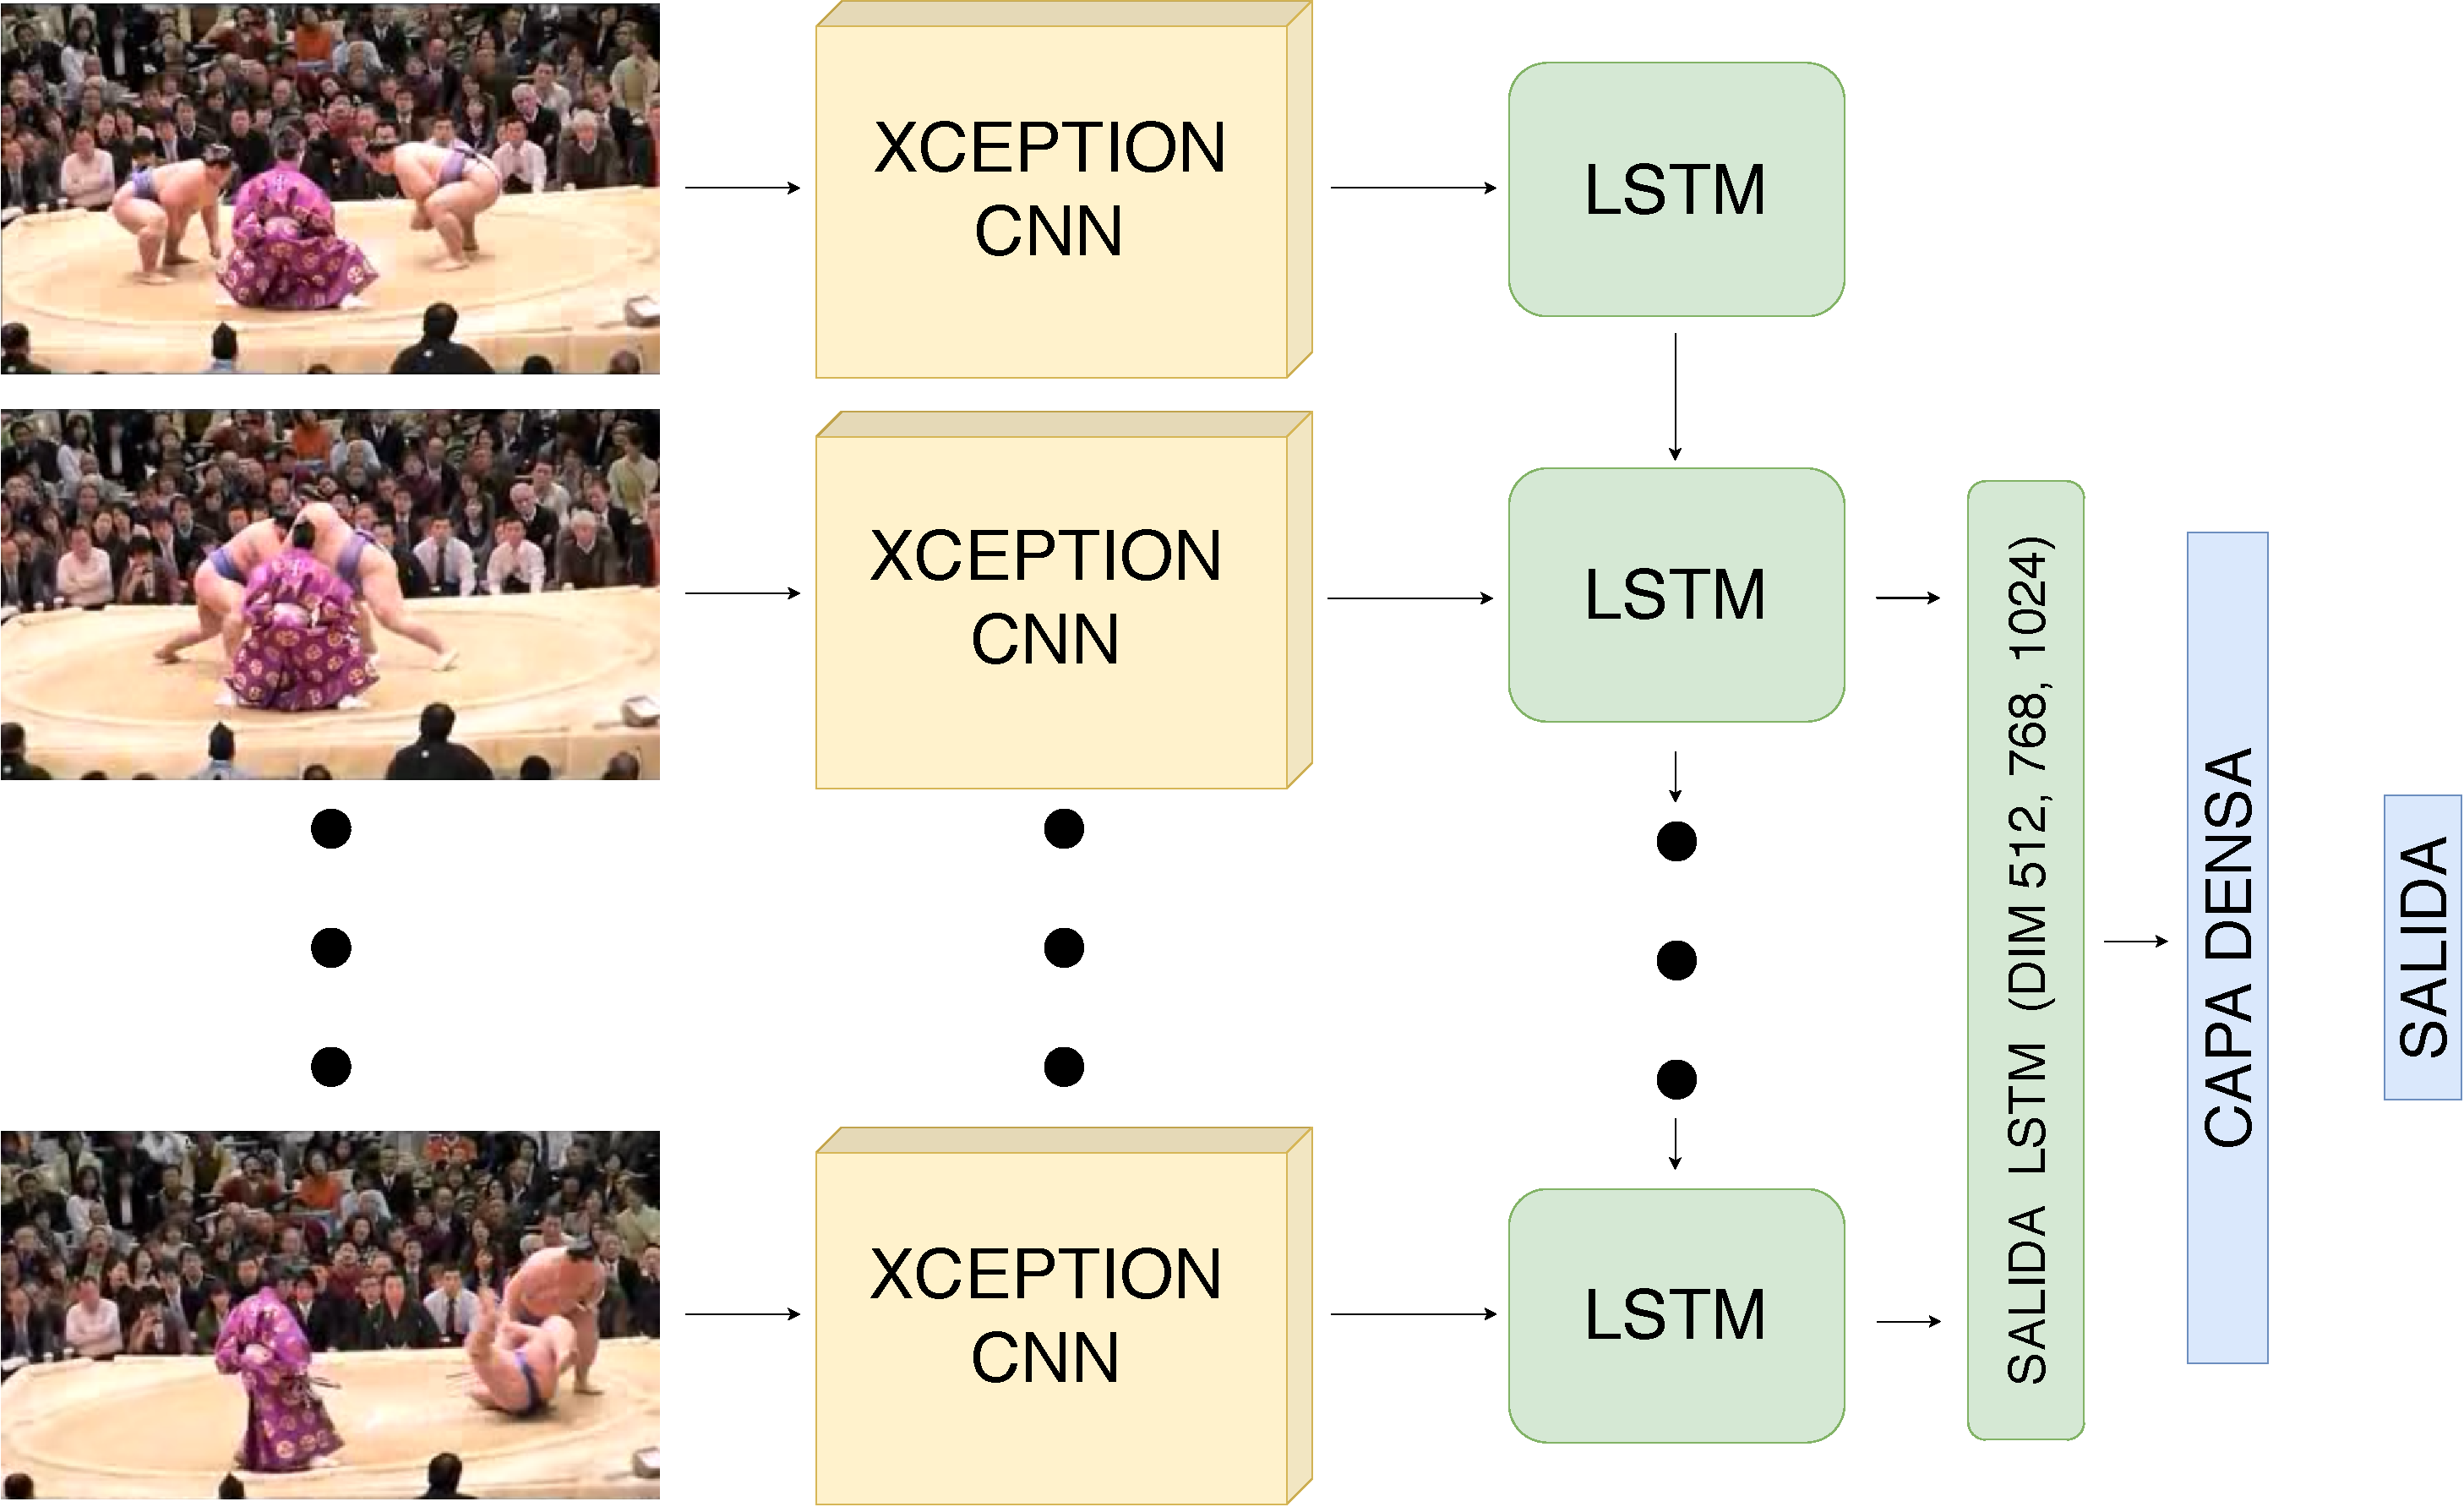
\includegraphics[width=.9\textwidth]{images/cnn_lstm.pdf}
  \caption{Extractor de características propuesto, junto con las capas
    completamente conectadas para el entrenamiento. Una vez el modelo
    ha sido preentrenado en el conjunto UCF-101, se eliminan las capas
    completamente conectadas. Por tanto, nuestro extractor de
    características final está compuesto por réplicas de la red
    Xception para cada uno de los fotogramas de entrada, y una red
    LSTM con tamaño de salida 512, 768 o 1024, que será lo que
    conoceremos como descriptor del fragmento de vídeo.}
  \label{fig:cnn-lstm}
\end{figure}

\subsection{Arquitectura detectora de anomalías completa}

Una vez ha sido preentrenado el extractor de características,
procedemos al entrenamiento del modelo completo. Manteniendo estática
la red extractora y eliminando toda la parte completamente conectada
de dicho modelo, calculamos los descriptores para los fragmentos de
vídeo. Con dichos fragmentos, haciendo la interpolación que proponen
en el modelo original, obtenemos la representación de tamaño fijo para
cada vídeo del conjunto de datos. Con dichas representaciones,
entrenamos un clasificador completamente conectado utilizando la función
de pérdida multi-instancia propuesta en el artículo.\\

Una vez tenemos el clasificador completamente conectado, construimos
el modelo final. Dicho modelo está compuesto por el extractor de
características hasta la salida de la red LSTM, seguido por la red
completamente conectada.

\end{document}

%%% Local Variables:
%%% mode: latex
%%% TeX-master: "../main"
%%% End:
